% arXiv: build with pdflatex; tectonic (XeTeX) defines \pdfoutput too, so skip it there.
\ifdefined\XeTeXversion\else\pdfoutput=1\fi
\documentclass[10pt,letterpaper]{article}

\usepackage[utf8]{inputenc}
\usepackage[T1]{fontenc}
\usepackage{newtxtext}
\renewcommand{\ttdefault}{lmtt}
\usepackage{amsmath,amssymb,amsthm}
\usepackage[varvw]{newtxmath}
\usepackage[letterpaper,margin=1in]{geometry}
\usepackage{microtype}
\usepackage{graphicx}
\usepackage{booktabs}
\usepackage{adjustbox}
\usepackage{longtable}
\usepackage{float}
\usepackage{array}
\setlength{\parskip}{2pt plus 1pt}
\usepackage{enumitem}
\usepackage[font=small]{caption}
\setlist{nosep,leftmargin=*}
\usepackage[round,semicolon,authoryear]{natbib}
\usepackage{url}
\usepackage{xcolor}
\usepackage{hyperref}

\newcommand{\papertitle}{Learning a calibrated decision head from logged bandit feedback}
\newcommand{\paperkeywords}{logged bandit feedback, calibration, proper scoring rules, decision heads, selective classification, LoRA}

\hypersetup{
  colorlinks=true,
  linkcolor={blue!60!black},
  citecolor={green!40!black},
  urlcolor={blue!70!black},
  pdftitle={\papertitle},
  pdfauthor={NAME},
  pdfsubject={Machine learning},
  pdfkeywords={\paperkeywords}
}

\theoremstyle{plain}
\newtheorem{corollary}{Corollary}

\setlength{\emergencystretch}{3em}

\title{\papertitle}
\author{NAME\\
  AFFILIATION\\
  \texttt{EMAIL}}
\date{}

\setlength{\textfloatsep}{10pt plus 2pt minus 4pt}
\setlength{\intextsep}{8pt plus 2pt minus 2pt}
\begin{document}
\maketitle
\begin{abstract}
A decision head reads a state and a list of options and returns a probability for each option in one forward pass; a caller answers when the top probability clears a threshold and escalates otherwise. Once deployed, it usually observes only whether the option it chose was right: logged bandit feedback. We adapt such a head, a LoRA adapter on Qwen3-0.6B-Base and 1.7B-Base, from that feedback, and report three results.

First, a proper score of the sampled action's own probability is not a usable REINFORCE reward. That a detached, parameter-dependent reward drops the pathwise term of the gradient is known; we give the corollary for this reward: against a group-mean baseline every wrong action earns at least the gold action's reward, the lowest-probability wrong action sampled gets the largest advantage, and at $K = 2$ the signal is exactly zero. In practice it cut one score task's accuracy from .636 to .111.

Second, with full labels, no bandit objective beat cross-entropy plus one temperature on calibration under label-space shift; the best arm was level, $-$.002 [$-$.006, +.004]. This replicates a concurrent finding under a stricter protocol: transfer to unseen label schemas, a continued cross-entropy control, and four bandit arms under one temperature.

Third, from logged bandit feedback alone, Chosen-Action Proper Scoring (CAPS), the direct method with a proper score that fits the chosen action's probability to its logged outcome by the pathwise gradient, beats fine-tuning on confirmed answers only, which is positive-unlabeled learning with the negatives discarded: on Banking77 by +2.6 points [1.9, 3.3] in accuracy, .053 in ECE and .0095 in AURC. It stays 1.5 points [1.0, 2.0] below full-label training at 0.6B and .6 points [.2, 1.1] below it at 1.7B, so the gap shrinks with scale (three CAPS seeds, one full-label seed at 1.7B), and propensity weights add nothing, as expected of a well-specified regression. Under feedback flipped at a known rate, CAPS calibrates to the noisy channel without any correction, backward correction recovers most of the clean calibration, and early stopping on the held-out log-likelihood of logged outcomes prevents the memorisation of the single noisy draw.
\end{abstract}

\noindent\textbf{Keywords:} \paperkeywords

\section{Introduction}\label{sec:1}

\textbf{The decision head.} A decision head answers typed questions about a text state: yes or no, one of K options, or a level on a scale. The options are part of each request, so the same model answers label sets it was never trained on. It returns a full distribution per question from the option-letter probabilities at an answer slot, in one forward pass, with no text generated. The caller's code turns the probabilities into actions, for example by answering above a confidence threshold and escalating below it, which is selective classification with a reject option. That only works if the probabilities are calibrated and rank the errors lowest. Ours is a LoRA adapter on Qwen3-0.6B-Base and 1.7B-Base. Its in-domain ECE is .013 to .015, but it is overconfident on unfamiliar schemas, with ECE up to .22. The setting is the one TypeSafe AI announced with Jev \citep{typesafe2026jev}, trained by an unpublished recipe called RLCD, reinforcement learning for calibrated decisions. Our decision head is an independent re-implementation of the concept; jevmark is the name of its code repository and released adapters.

\textbf{Why logged bandit feedback is the realistic case.} After deployment on a new domain, labels are expensive and rare. What a system does record is whether the action it took turned out right: a ticket reopened or not, a routing corrected or not. This is logged bandit feedback: one outcome per interaction, only for the chosen action, under a known logging policy. The common practice is to fine-tune on the interactions that went well and discard the rest. That discards the negatives, which makes it positive-unlabeled learning, and, as we show, leaves the model overconfident (Section~\ref{sec:4.3}).

\textbf{This paper.} It makes three claims, the third of which is the core.
\begin{enumerate}
  \item \textbf{A corollary on detached proper-score rewards.} The general principle is that a detached, parameter-dependent reward drops the pathwise term of the gradient \citep{schulman2015scg,mohamed2020montecarlo}. Our contribution is the specific algebra when the reward is a proper score of the sampled action's own probability: a wrong action's reward is never below gold's, the lowest-probability wrong action sampled gets the largest advantage, and the signal is exactly zero at $K = 2$ (Section~\ref{sec:3}); and the measured collapse (Section~\ref{sec:4.2}). The concurrent OpenJev-RLCD \citep{gao2026openjev} reaches the same recipe, pathwise gradient only and the score-function term harmful, by a gradient-norm argument for a different object: its REINFORCE term acts on a sampled rationale, not on the answer whose probability is scored. \citet{bereket2025uncalibrated} and \citet{damani2025rlcr} show that REINFORCE with a proper-score reward works when the forecast is a separately emitted probability, and \citeauthor{bereket2025uncalibrated} trace GRPO's overconfidence to dividing the advantage by the group standard deviation. Our group baseline subtracts the group mean only, with no standard-deviation normalisation (\texttt{rlcd.normalize\_std: false} in every full-label run, and a batch mean only in the logged-feedback REINFORCE arm), so their failure mode does not apply, and our pathology is specific to scoring the sampling probability itself.
  \item \textbf{A replication, under a stricter protocol, that full labels leave nothing for bandit objectives.} OpenJev-RLCD's direct-scorer ablation reports that proper-score RL never beat cross-entropy on CLINC150 (94.6 against 96.3 accuracy) and that RLVR collapsed to the mode. We find the same direction and add the transfer-to-unseen-schema protocol, the continued cross-entropy control, four bandit arms under one temperature, and the finding that a single temperature is the strongest cheap fix (Section~\ref{sec:4.2}). The direction is not new.
  \item \textbf{Learning from logged bandit feedback with CAPS.} CAPS is the direct method of logged bandit feedback \citep{dudik2011doubly}, trained with a proper score on the chosen action, the regression-oracle objective \citep{foster2018regcb,foster2020squarecb}. What is new is the package for LoRA-adapted LLM decision heads at 2000 interactions:
  \begin{itemize}
    \item positive-only fine-tuning diagnosed as positive-unlabeled learning \citep{elkan2008pu} and beaten from 2000 interactions on Banking77 and from 500 on emotion, with better calibration and selective risk at every log size;
    \item no gain from propensity weights, the expected behaviour of a well-specified regression \citep{shimodaira2000covariate,byrd2019importance};
    \item calibration to the noisy channel without correction, and backward correction \citep{natarajan2013noisy,patrini2017losscorrection} with its $1/(1-2f)$ factor \citep{angluin1988noisy};
    \item memorisation of a fixed noisy log, and checkpoint selection on the held-out log-likelihood of logged outcomes, which needs no label.
  \end{itemize}
\end{enumerate}

\textbf{What the paper does not show.} The feedback is simulated from gold labels, cleanly or with symmetric flips at a known rate, on two adaptation domains, Banking77 and emotion, with one log each, and at 1.7B CAPS has three training seeds and the baselines one. There is no counterfactual-risk policy learner (POEM or BanditNet), no doubly robust arm and no off-policy value estimate of the learned policy (Section~\ref{sec:5}). The gap to full labels does not shrink as the log grows.

\section{Related work}\label{sec:2}

\textbf{Calibrated decision heads for agents.} Jev \citep{typesafe2026jev} and the other published reconstruction, OpenJev-RLCD \citep{gao2026openjev}, answer typed questions about a state in one forward pass, with a confidence the caller thresholds. Their use is the cascade, in which a cheap model answers what it is sure of and defers the rest \citep{chen2023frugalgpt}, and confidence trained into the small model gives the better deferral trade-off \citep{chuang2025selfref}. Thresholding the top posterior is selective classification \citep{geifman2017selective}, so we evaluate the caller by its risk-coverage curve. Option-letter readout has known position and order biases \citep{zheng2024selectors}, so we randomise option order in every split and report accuracy by gold letter position (R1, Section~3); unlike a confidence stated in words \citep{xiong2024uncertainty}, ours is the distribution over the options the head read, with no text generated.

\textbf{Learning from logged bandit feedback.} CAPS is the direct method of logged bandit feedback \citep{dudik2011doubly} and the regression-oracle objective \citep{foster2018regcb,foster2020squarecb}, which a contextual-bandit bake-off found competitive without propensity weights \citep{bietti2021bakeoff}. Counterfactual risk minimisation instead weights the policy objective by inverse propensities, with variance penalties, self-normalisation and clipping \citep{swaminathan2015crm,swaminathan2015selfnormalized,joachims2018banditnet}; doubly robust estimators combine the two \citep{dudik2011doubly}, and simulating bandit feedback from a labelled multiclass dataset is the standard protocol \citep{beygelzimer2009offset}. Importance weights are unnecessary for a well-specified conditional model \citep{shimodaira2000covariate} and have little effect on deep networks trained to convergence \citep{byrd2019importance}. Fine-tuning on confirmed answers only is positive-unlabeled learning, which recovers the posterior only up to a constant \citep{elkan2008pu}, and the decision-head form of self-training on filtered successes \citep{zelikman2022star}.

\textbf{Proper scoring rules as losses and as rewards.} A strictly proper score is minimised in expectation by the true probability \citep{brier1950verification,gneiting2007proper}, which makes it a calibration-respecting loss and, when the forecast is a separately emitted probability, a sound reward. Binned ECE \citep{naeini2015ece} is biased, which is why we report Brier and NLL beside it \citep{nixon2019measuring}, and one temperature repairs calibration post hoc \citep{guo2017calibration}. As RL rewards on a verbalized confidence, proper scores yield calibrated models \citep{damani2025rlcr}, and \citet{bereket2025uncalibrated} show that the estimator, not the score, then decides calibration: an unbiased group baseline gives calibrated forecasts and GRPO's standard-deviation normalisation drives them to the extremes.

\textbf{Calibration in RL for language models and the gradient question.} That a detached, parameter-dependent reward drops the pathwise term of the gradient is the general rule of stochastic computation graphs \citep{schulman2015scg,mohamed2020montecarlo}; our first result is its corollary for a proper score of the sampled action's own probability under REINFORCE \citep{williams1992reinforce} with the group baseline of GRPO \citep{shao2024deepseekmath}, and outcome-only rewards degrade calibration \citep{damani2025rlcr}. OpenJev-RLCD \citep{gao2026openjev} optimises the readout distribution by the pathwise gradient of a proper score, its deterministic policy gradient with respect to the reported distribution, and finds the score-function term, which acts on a sampled rationale, at 7 to 12 times the pathwise term's gradient norm and more of it monotonically worse. Its direct-scorer ablation reports that proper-score RL never beat cross-entropy on CLINC150 (94.6 against 96.3) and that RLVR collapsed to the mode; our second result agrees under a transfer protocol with a continued cross-entropy control.

\textbf{Noisy feedback.} Feedback flipped at a known rate $f$ is random classification noise on the outcome \citep{angluin1988noisy}; the observed outcome rate $f + (1-2f)\,P(\mathrm{correct})$ that CAPS fits is the symmetric case of the class-conditional identity, with the clean posterior an affine transform of the corrupted one \citep{natarajan2013noisy,menon2015corrupted}, and inverting it is backward correction with a known transition matrix \citep{patrini2017losscorrection}, whose error grows by the $1/(1-2f)$ factor of \citeauthor{angluin1988noisy}. \citet{agarwal2021noisybandit} study flipped bandit feedback with a known rate for an online linear learner; networks memorise noisy labels given enough passes \citep{zhang2017rethinking}, and early stopping is the provable remedy \citep{li2020earlystopping}.

\textbf{Calibration under shift and after fine-tuning.} A single temperature is strong in-domain and fragile under shift \citep{ovadia2019shift}. Our second result says the bandit alternatives are no less fragile on unseen label schemas. LoRA forgets less than full fine-tuning but still forgets \citep{biderman2024lora}, so we report forgetting on the original domain.

\textbf{Dataset quality and evaluation hygiene.} Our leak probes are leakage detection by exploratory models on non-target features \citep{kaufman2012leakage} against a permutation null \citep{ojala2010permutation}. Benchmark test sets contain label errors \citep{northcutt2021pervasive}; for Banking77, \citet{ying2022banking77errors} flag about 1,400 of 13,083 utterances, about 11 percent, in line with our audit's .12 and .14. The emotion dataset is distantly supervised from hashtags \citep{saravia2018carer}, which human validation puts at about 90 percent label accuracy \citep{abdulmageed2017emonet}; our audit finds a problem in a third of a uniform sample.

\section{Method: Chosen-Action Proper Scoring}\label{sec:3}

\textbf{Setting.} A logged interaction is $(x, O, a, q(a \mid x), r)$: $x$ is a state and $O$ its $K$ options, $a$ is the action the logging policy $q$ chose and $q(a \mid x)$ its logging propensity, recorded exactly, and $r \in \{0, 1\}$ records whether $a$ was right.

The learner starts from a general decision head $p_\theta$ and sees only the log. In our experiments $q = 0.9\, p_0 + 0.1/K$, epsilon-greedy over the starting model $p_0$, so every option has support.

\textbf{Objective.} CAPS minimises
\begin{equation}
  \label{eq:caps}
  L(\theta) = \mathbb{E}_x\, \mathbb{E}_{a \sim q(\cdot \mid x)} \bigl[ S\bigl(p_\theta(a \mid x), r(x, a)\bigr) \bigr]
\end{equation}
with $S$ a strictly proper binary score: Brier, $(r - p)^2$, by default, or the log score. The empirical mean over the log estimates $L$ directly. The gradient is the pathwise gradient through $p_a$; for Brier it is $-2 (r - p_a)\, \partial p_a / \partial \theta$. A right action is pushed up and a wrong one down.

\textbf{Identity.} CAPS is the direct method of \citet{dudik2011doubly}, with a proper score as the regression loss on the chosen action's outcome and the argmax of the fitted head as the policy, and it is OpenJev-RLCD's stage 1 specialised to partial feedback: where stage 1 scores the whole readout distribution against the one-hot label, CAPS scores the one component the log reveals, the chosen action's probability against its own outcome.

\textbf{Why no propensity weight.} For each $(x, a)$ with $q(a \mid x) > 0$, the inner term is minimised at $p(a \mid x) = P(r = 1 \mid x, a)$, whatever $q$ is. The target does not depend on the logging policy as long as it has support, so the unweighted fit is consistent for a well-specified model \citep{shimodaira2000covariate}. The propensity only sets how a finite model trades errors between actions, and $L$ makes that trade as the deployed policy acts. A weight $1/q$ would retarget it to a uniform average over options.

Accuracy is a consequence, not the objective: moving right actions up and wrong ones down moves the argmax, and options the logger never takes are unconstrained. A negative on an option other than the logger's top choice arises only from the logger's randomness; on our main log, 1514 of 2593 negatives (.584) fall on such options, and about .545 of those come from the uniform exploration term.

\begin{corollary}[A proper score of the sampled action's probability as a detached reward]\label{cor:detached}
Take $K$ options, gold $g$, and a proper score used as the reward of the sampled action: Brier, $R(a) = 1 - (r_a - p_a)^2$, or the log score, $R(a) = r_a \log p_a + (1 - r_a) \log(1 - p_a)$.

The gradient of the expected reward, $\sum_a p_a R(a)$, has a score-function term, $\sum_a R(a)\, \nabla p_a$, and a pathwise term, $\sum_a p_a \nabla R(a)$. Detaching $R$ keeps only the first \citep{schulman2015scg}. Form REINFORCE advantages against the mean of a sampled group, the sample itself included and not divided by the group standard deviation.

(i) If $K > 2$, every wrong action's reward is at least gold's. In each group, the lowest-probability wrong action sampled has the largest reward, so its advantage is non-negative. Whenever the group also samples gold, gold's advantage is non-positive.

(ii) If $K = 2$, all rewards in every group are equal, and the gradient is zero.
\end{corollary}

\begin{proof}
A wrong action $w$ has $r_w = 0$ and $p_w \le 1 - p_g$. Under Brier, $R(w) = 1 - p_w^2$ and $R(g) = 1 - (1 - p_g)^2$; under the log score, $R(w) = \log(1 - p_w)$ and $R(g) = \log p_g$. Both rewards decrease in $p_w$ and equal $R(g)$ at $p_w = 1 - p_g$. Hence $R(w) \ge R(g)$, and the smallest sampled $p_w$ gives the group maximum. At $K = 2$, $p_w = 1 - p_g$ exactly, so $R(w) = R(g)$.
\end{proof}

The score grades $p_a$ as a forecast of $r_a$, and a low probability on a wrong option is always a good forecast; CAPS uses the same score as a loss on $p_a$ by its pathwise gradient, not as a reward on $a$. Neither statement depends on the standard-deviation normalisation that \citet{bereket2025uncalibrated} identify as GRPO's source of overconfidence, since our group of 4 and the logged-feedback REINFORCE arm subtract the mean only (Appendix~\ref{sec:setup}), and the corollary does not contradict proper-score rewards on a confidence the model emits separately \citep{damani2025rlcr,bereket2025uncalibrated}, only on the probability with which it sampled the rewarded action.

\textbf{Selection.} Train on the first $0.9N$ interactions. Keep the checkpoint, from a 50-step grid, with the highest mean Bernoulli log-likelihood of the logged outcomes under $p(\text{logged action})$ on the last $0.1N$: early stopping on the held-out log score of logged outcomes. No gold label is read. Under noisy feedback this is what prevents memorisation (Section~\ref{sec:4.3}).

\section{Experiments}\label{sec:4}

\subsection{Setup}\label{sec:4.1}

\textbf{Model and data.} The decision head is Qwen3-0.6B-Base or 1.7B-Base with LoRA \citep{hu2022lora,qwen2025qwen3}, read from the letter logits at each question's answer slot. It is trained with supervision on CLINC150 intents \citep{larson2019clinc} and SST-5 sentiment \citep{socher2013sst} and evaluated on 20 held-out intents and four schemas never trained on: AG News, Yelp \citep{zhang2015charcnn}, emotion \citep{saravia2018carer} and Banking77 \citep{casanueva2020banking77}. Training details and the data gates are in Appendix~\ref{sec:setup}.

\textbf{Adaptation protocol.} The 0.6B model logs every message of the Banking77 train split once, 9942 messages, each a 10-option choice with gold always present, sampling from $q = 0.9\,p + 0.1/K$ and recording only the correctness of its action; policy accuracy is .836 and the outcome rate .739. Learners see the first $N \in \{500, 2000, 5000\}$ interactions at equal steps; at N 5000, CAPS-Brier, CAPS-log and \texttt{full\_sft} each have three training seeds, and CAPS-Brier also has a second log draw. Evaluation is on the full Banking77 test split (3080 records), plus \texttt{test\_indomain} and \texttt{test\_unseen\_intents} for forgetting, with paired 95 percent record-bootstrap intervals \citep{efron1979bootstrap,efron1993introduction}.

\textbf{Learners.} The temperature learner fits one temperature to the logged outcomes and changes no argmax; \texttt{positive\_sft} is cross-entropy on confirmed actions, positive-unlabeled learning with the negatives discarded, and what practitioners do; \texttt{full\_sft} is cross-entropy on gold for every logged interaction, the upper bound. Three off-policy forms on the same log use the propensities, \texttt{outcome\_minus\_p\_log}, \texttt{ips\_log} and \texttt{ips\_positive} (Appendix~\ref{sec:setup}); they are not counterfactual risk minimisation, which weights the policy objective itself and was not run (Section~\ref{sec:5}). In tables, CAPS with the Brier score is the run name \texttt{direct\_brier}, and with the log score \texttt{direct\_log}.

\textbf{Metrics.} Accuracy, ECE with 15 equal-width bins, Brier and NLL, and two selective-classification metrics for the caller who thresholds \citep{geifman2017selective}, with questions ranked by top-1 probability: AURC, the area under the risk-coverage curve, and Cov@eps, the largest share of questions a top-1 threshold keeps with error at most eps (Appendix~\ref{sec:setup}). Lower AURC and higher Cov@eps are better, and the tables show Cov@.05.

A temperature changes the level of the probabilities and only slightly their ranking: at N 5000 the temperature learner cuts zero-shot ECE from .063 to .020 but moves AURC only from .0333 to .0328 (Table~\ref{tab:A1}; details in Appendix~\ref{sec:A1}).

\subsection{Full labels: the negative results (v2)}\label{sec:4.2}

A first run used Brier as a detached REINFORCE reward on fully labelled in-domain data, with a group of 4 and a mean baseline without standard-deviation normalisation. Score accuracy fell from .636 to .111 on SST-5 and from .505 to .044 on Yelp, and a simulation of the sampler on the SFT model lowered the gold logit in 24.0 percent of questions and raised it in 1.8 percent: the corollary of Section~\ref{sec:3} at work. Five arms, from continued cross-entropy to CAPS with the log score, then ran three seeds each at 0.6B on full labels (Table~\ref{tab:A6}). Against SFT plus one in-domain temperature, at unseen-schema mean ECE .121, every arm's unseen-schema ECE is higher, by +.031 to +.127, and given its own temperature the best arm and the control are only level (Figure~\ref{fig:v2_arm_ece}). When gold is known, whether a sampled answer was right carries no more than the label itself, and one temperature is the strongest cheap fix. OpenJev-RLCD reports the same direction on CLINC150 with a different training setup; the transfer to unseen schemas and the continued cross-entropy control are ours.

\begin{figure}[t]
\centering
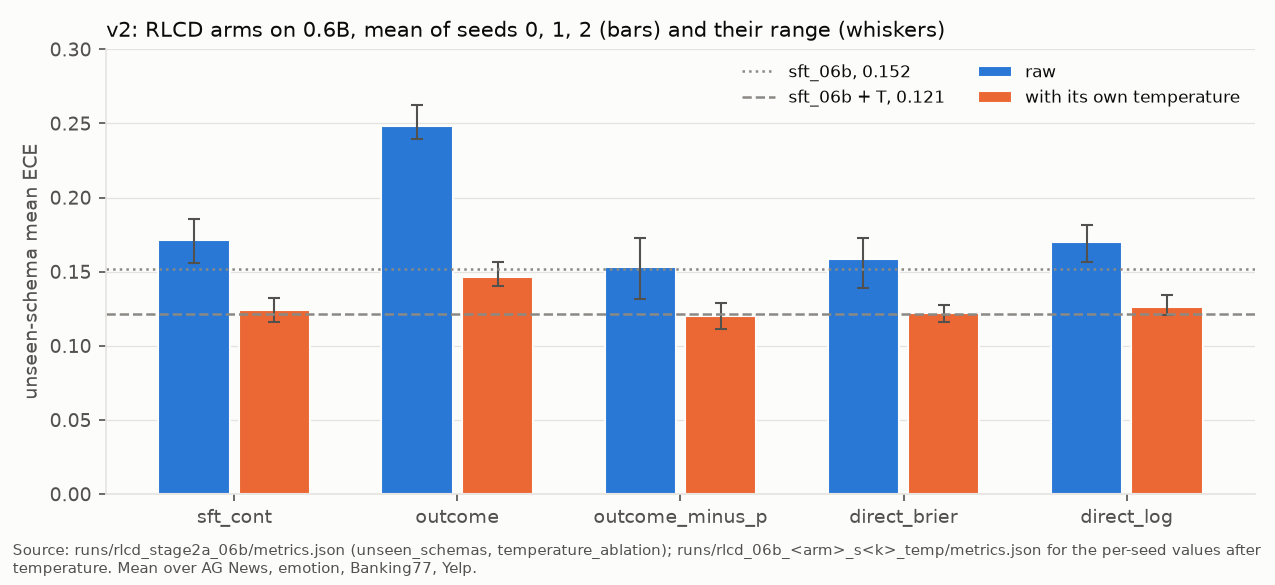
\includegraphics[width=0.6\textwidth]{figures/v2_arm_ece.png}
\caption{Unseen-schema mean ECE per full-label arm, 0.6B, mean of three seeds with their range, raw and with its own temperature, against SFT and SFT plus one temperature. Provenance: Table~\ref{tab:prov}, F1.}\label{fig:v2_arm_ece}
\end{figure}

\subsection{Logged bandit feedback only (v3, Banking77)}\label{sec:4.3}

\textbf{The N-curve.} From 2000 interactions CAPS-Brier beats \texttt{positive\_sft}: it ties at N 500, +.002 [$-$.006, +.009], and leads by +.027 [+.019, +.035] at N 2000 and +.024 [+.016, +.031] at N 5000, with ECE lower by .052 to .060 and AURC by .0035 to .0099 at every N, and Cov@.05 level at N 500 and higher by +.065 [+.048, +.093] and +.069 [+.046, +.094] at N 2000 and 5000 (Figure~\ref{fig:v3_n_curve}; Table~\ref{tab:A1}). It stays 0.7 to 1.8 points below \texttt{full\_sft} in accuracy and .0026 to .0047 above it in AURC. The temperature learner keeps zero-shot accuracy (.851) and has the lowest or joint-lowest ECE, .020 at N 5000, but its Brier, NLL and AURC stay far above every trained learner's.

\begin{figure}[t]
\centering
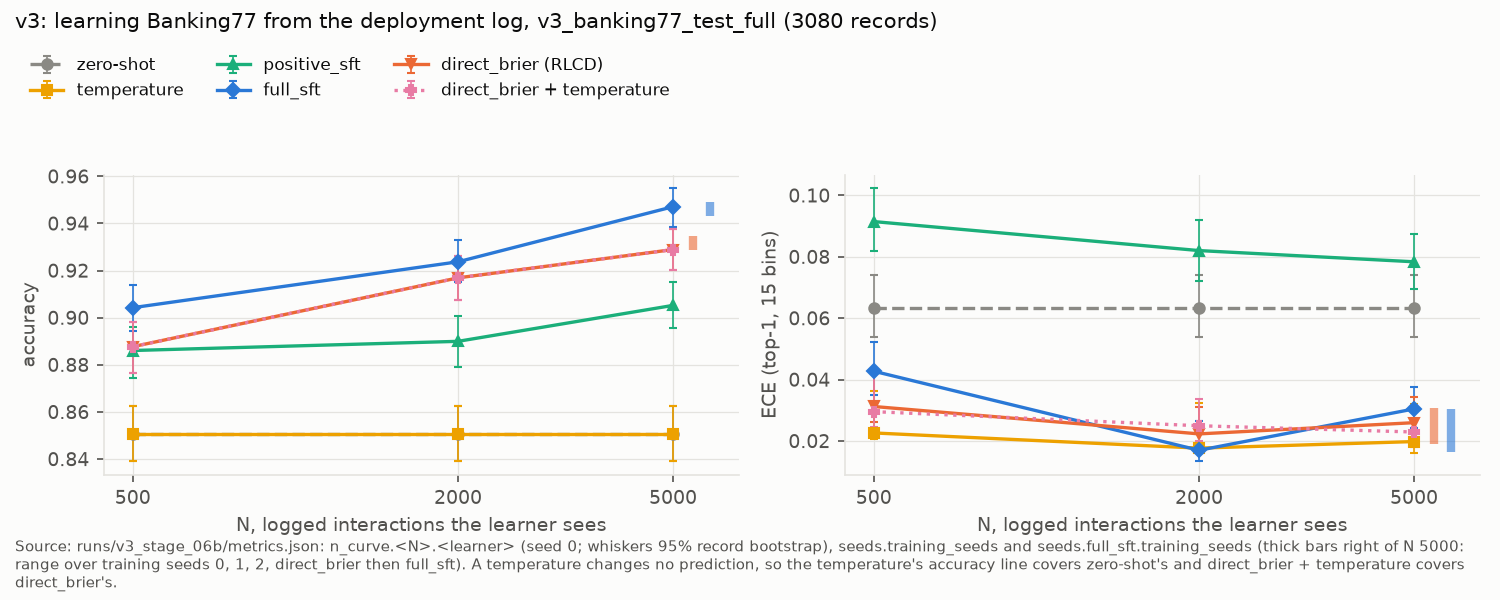
\includegraphics[width=0.6\textwidth]{figures/v3_n_curve.png}
\caption{Accuracy and ECE against N on the Banking77 test split, 0.6B: every learner at seed 0 with 95 percent record-bootstrap intervals, and at N 5000 the range over three training seeds for CAPS-Brier (\texttt{direct\_brier}) and \texttt{full\_sft}. Provenance: Table~\ref{tab:prov}, F2.}\label{fig:v3_n_curve}
\end{figure}

\textbf{Seeds.} Over three training seeds at N 5000, CAPS-Brier is +.026 [+.019, +.033] over \texttt{positive\_sft} in accuracy and $-$.0095 [$-$.0121, $-$.0070] in AURC, and $-$.015 [$-$.020, $-$.010] below \texttt{full\_sft}'s seed mean, with ECE level, +.003 [$-$.001, +.008] (Table~\ref{tab:A2}). Training seeds and the second log draw move accuracy by at most .6 points, and a temperature fitted on CAPS-Brier's own training interactions comes out near 1 and moves ECE by at most .003 (Appendix~\ref{sec:A2}).

\textbf{Off-policy baselines.} Propensity weights add nothing: \texttt{ips\_positive} equals \texttt{positive\_sft}, +.000 [$-$.003, +.004] in accuracy at N 5000, and no off-policy arm beats CAPS-Brier on accuracy with an interval excluding 0 (Table~\ref{tab:A3}). With full support and a well-specified regression target, this is the expected result. The log score in place of Brier is a choice within the same family: over three seeds CAPS-log is +.002 [$-$.001, +.005] in accuracy and $-$.020 [$-$.029, $-$.010] in NLL against CAPS-Brier, but it forgets more in-domain and is behind at N 2000 on one seed, so Brier stays the default (Appendix~\ref{sec:A3}).

\textbf{Noisy feedback.} With outcomes flipped at $f \in \{0.1, 0.2, 0.3\}$, with nested draws, CAPS learns the noisy posterior $p = f + (1-2f)\,P(\mathrm{correct})$ without correction: the selected run at f 0.2 has mean top-1 .743 against a channel line of .744 (Figure~\ref{fig:v4_noise_sweep}; Table~\ref{tab:A4}). Backward correction, $(p - f)/(1 - 2f)$ on the top-1 probability, gives ECE against correctness of .020, .051 and .068 at f 0.1, 0.2 and 0.3, against the clean run's .026; the amplification $1/(1 - 2f)$ is 1.25, 1.67 and 2.5. Its accuracy loss grows with f, $-$.006, $-$.022 and $-$.041, and is smaller than \texttt{positive\_sft}'s at 0.1 and 0.2 and level at 0.3, $-$.003 [$-$.014, +.007], one seed per rate. Trained to the end, CAPS memorises the single flip draw and falls to .734 at 0.3, below zero-shot's .851, while early stopping on the held-out log score of logged outcomes picks steps before the collapse every time. A soft-target diagnostic shows that the residual is the variance of one noisy draw per interaction, not a limit of the objective (Appendix~\ref{sec:A4}).

\begin{figure}[t]
\centering
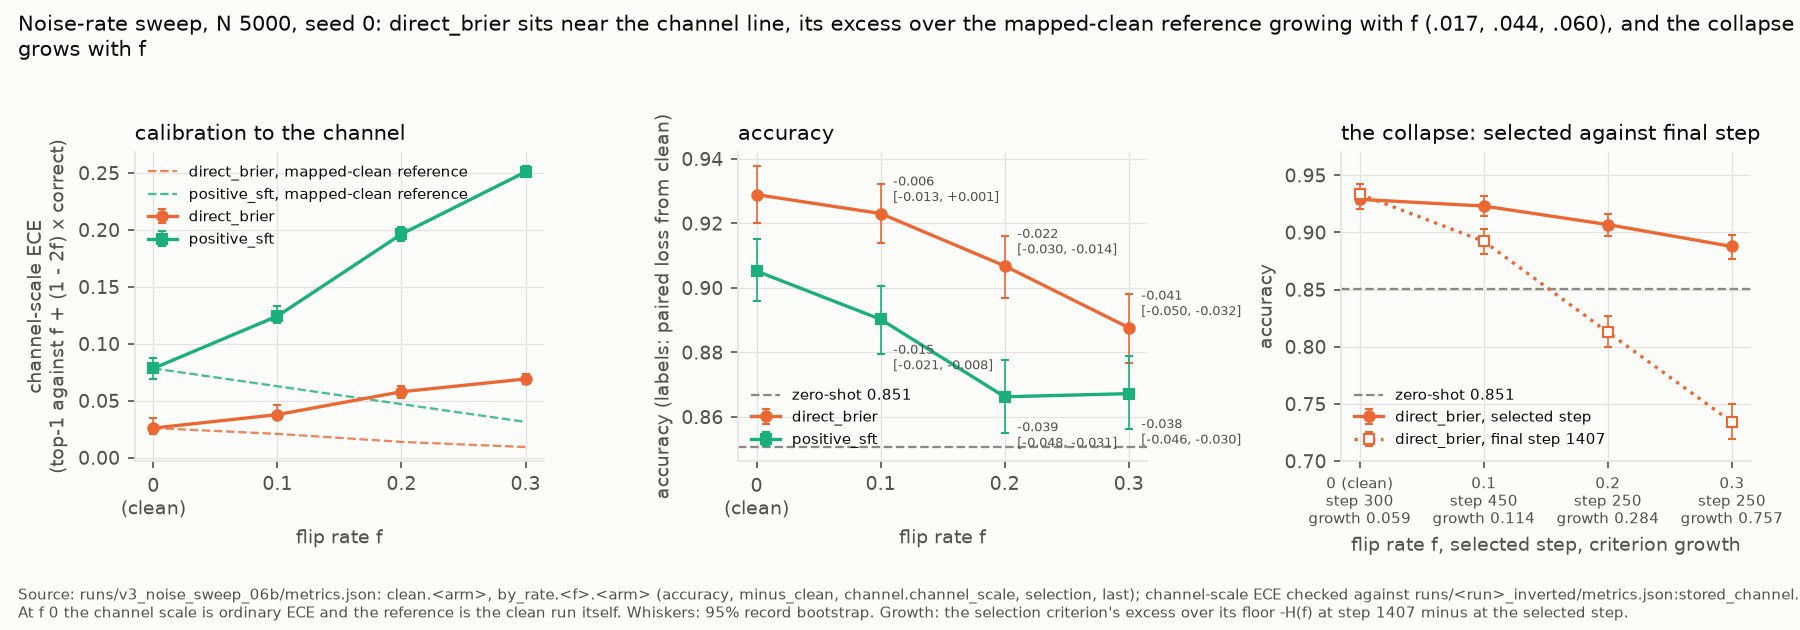
\includegraphics[width=\textwidth]{figures/v4_noise_sweep.png}
\caption{Noise-rate sweep, N 5000, seed 0: calibration to the channel, accuracy, and the selected step against the final step. Provenance: Table~\ref{tab:prov}, F4.}\label{fig:v4_noise_sweep}
\end{figure}

\textbf{Scale.} At 1.7B, with its own log, CAPS-Brier on three training seeds reaches accuracy .947 (.942, .949) and leads \texttt{positive\_sft} by +.034 [+.026, +.041], and against a single \texttt{full\_sft} seed its gap to full-label training shrinks to .6 points [.2, 1.1], $-$.006 [$-$.011, $-$.002], from 1.5 points [1.0, 2.0] at 0.6B (Figure~\ref{fig:v4_scale}; Table~\ref{tab:A5}). Every 1.7B CAPS-Brier seed is above every 0.6B one, so the larger model helps the learner from logged bandit feedback most.

\begin{figure}[t]
\centering
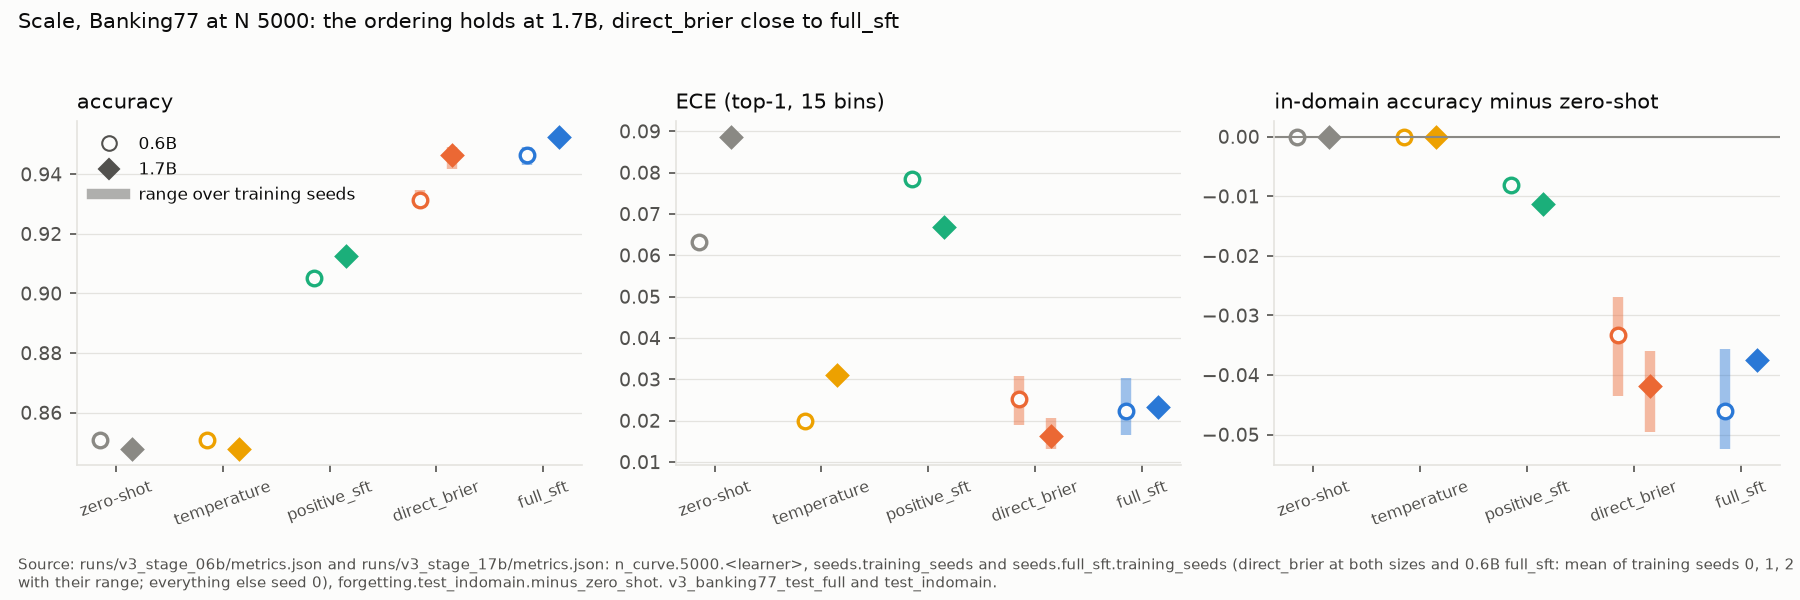
\includegraphics[width=\textwidth]{figures/v4_scale.png}
\caption{Scale, Banking77 at N 5000: 0.6B against 1.7B for every learner, with the range over training seeds where a size has more than one. Provenance: Table~\ref{tab:prov}, F5.}\label{fig:v4_scale}
\end{figure}

\textbf{Forgetting and selective prediction.} At N 5000, CAPS-Brier costs 2.7 to 4.3 points of in-domain accuracy across seeds and \texttt{full\_sft} 3.6 to 5.2, \texttt{positive\_sft} under 1, and CAPS-Brier keeps in-domain ECE within .010 of zero-shot. At a fixed confidence threshold of .95, \texttt{positive\_sft} keeps .916 of answers at .942 accuracy, so it passes on about 6 percent errors as confident, while CAPS-Brier keeps .743 at .986; at a fixed error budget of .05, CAPS-Brier keeps .957 of answers against \texttt{positive\_sft}'s .888. On the 500-record Banking77 subset, every CAPS-Brier run at N 5000 scores .926 to .936 from 5000 correctness bits, against gpt-4.1-mini's .918, with no paired interval.

\subsection{A second domain: emotion}\label{sec:4.4}

The emotion log domain is the dair-ai/emotion train split, 15958 messages, each a choice over all 6 labels with no \texttt{other} option. The same \texttt{sft\_06b} logs it at policy accuracy .542, so 8393 of the 15958 logged outcomes are negative, .526 computed from the stored counts, against $1 - .739 = .261$ on Banking77; evaluation is on the full emotion test split, 2000 records. CAPS-Brier leads \texttt{positive\_sft} at every N, by +.043 [+.027, +.060], +.126 [+.109, +.144] and +.217 [+.197, +.238] in accuracy at N 500, 2000 and 5000, with ECE lower by .186 to .276 (Figure~\ref{fig:v4_emotion_n_curve}; Table~\ref{tab:A7}). Over three seeds at N 5000 it is $-$.043 [$-$.056, $-$.031] below \texttt{full\_sft}'s one seed in accuracy, with ECE level, +.006 [$-$.005, +.018]. The per-N details, CAPS-log, the temperature learner, forgetting, the label ceiling and the API reference are in Appendix~\ref{sec:A7}.

Both predictions stated before these runs held. CAPS beats \texttt{positive\_sft} in accuracy and ECE on emotion from N 2000, as on Banking77, and in accuracy from N 500, where Banking77 tied; and the gap to \texttt{full\_sft} at N 5000 is larger than on Banking77, $-$.039 [$-$.052, $-$.027] against $-$.018 [$-$.025, $-$.011] on seed 0 and $-$.043 against $-$.015 for the seed means, as predicted from a harder task and a logging policy wrong more often, though the two change together, so the cause is not isolated. Not predicted was the size of the lead over \texttt{positive\_sft}, nine times Banking77's at N 5000: with fewer than half the outcomes positive, discarding the negatives discards most of the log.

\begin{figure}[t]
\centering
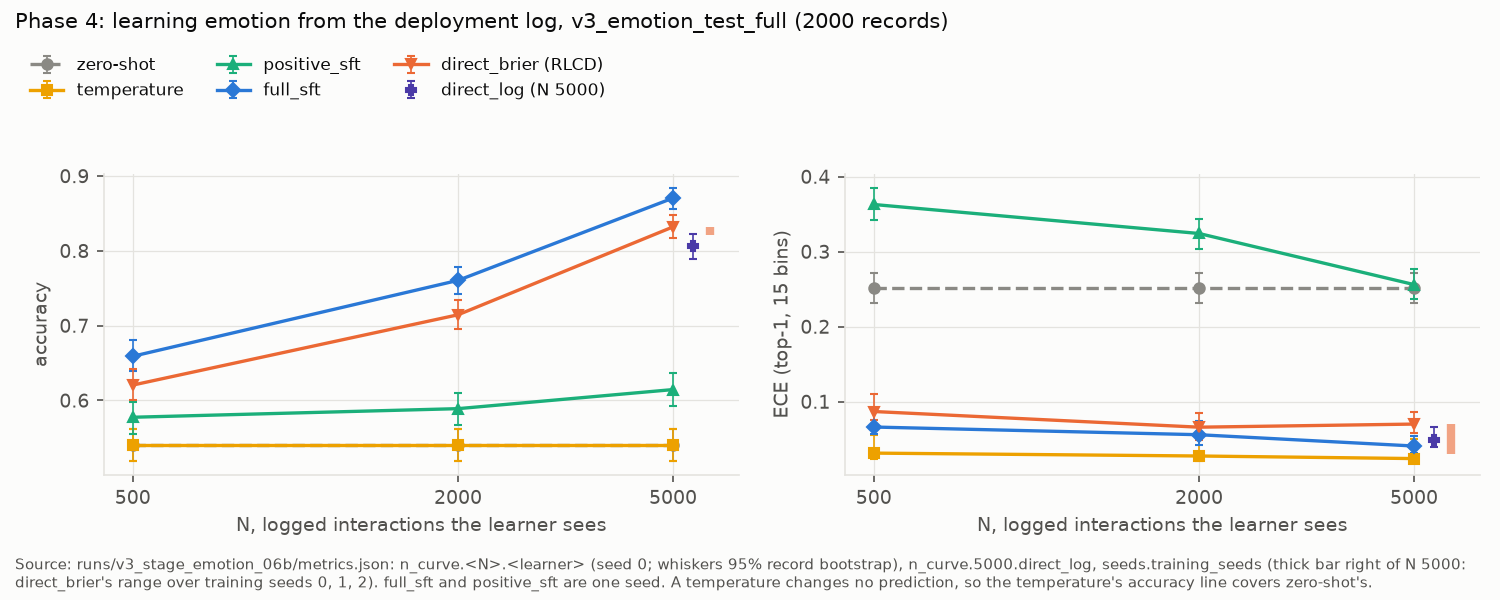
\includegraphics[width=0.6\textwidth]{figures/v4_emotion_n_curve.png}
\caption{Emotion N-curve, 0.6B, on the emotion test split: every learner at seed 0 with 95 percent record-bootstrap intervals, CAPS-log at N 5000, and CAPS-Brier's range over three training seeds. Provenance: Table~\ref{tab:prov}, F6.}\label{fig:v4_emotion_n_curve}
\end{figure}

\section{Limitations}\label{sec:5}

\begin{itemize}
  \item \textbf{Simulated feedback.} Outcomes come from gold labels, cleanly or flipped symmetrically at a known rate, while real feedback is delayed, biased towards some errors and of unknown noise rate, which backward correction needs; the compression towards the channel is global, with in-domain ECE up by .050 for the noisy run.
  \item \textbf{Domains and sizes.} There are two adaptation domains with one log each and one logging policy per domain at epsilon 0.1, .836 accurate on Banking77 and .542 on emotion; \texttt{positive\_sft} and \texttt{full\_sft} have one seed on emotion and at 1.7B, where CAPS-Brier has three, so those gaps carry no baseline seed variance; and the noise sweep has one seed per rate.
  \item \textbf{Missing off-policy arms.} The weighted arms reweight the direct-method loss; with no counterfactual-risk policy learner (POEM or BanditNet; \citealp{swaminathan2015crm,joachims2018banditnet}), doubly robust arm \citep{dudik2011doubly} or self-normalised estimate of the learned policy's value, the no-gain result is shown against reweighted regression, not against the methods built around the weights.
  \item \textbf{Label noise, judged by two language models, no human.} The judges find a label problem in .12 and .14 of a uniform Banking77 sample and in .32 and .40 of an emotion sample, and the clean feedback inherits these labels (Appendix~\ref{sec:setup}).
  \item \textbf{Selection.} Checkpoints are every 50 steps, so at N 2000, where the log-score arms peaked at the first candidate, a finer grid could favour them, and at N 500 only 50 interactions select.
  \item \textbf{Coverage of the claim.} The gap to full labels does not shrink with N, so the claim is that using failures beats discarding them, not that it replaces labels.
\end{itemize}

\section{Conclusion}\label{sec:6}

A decision head that can only see whether its chosen action was right should be fitted as the direct method with a proper score: the chosen action's probability against its own logged outcome, by the pathwise gradient. That is CAPS, OpenJev-RLCD's stage 1 restricted to the one component partial feedback reveals. With 2000 interactions it beats positive-only fine-tuning, which is positive-unlabeled learning with the negatives discarded, in accuracy, calibration and selective risk on both domains (Sections~\ref{sec:4.3} and~\ref{sec:4.4}), and on Banking77 it needs no propensity weights (Section~\ref{sec:4.3}); under feedback flipped at a known rate it learns the noisy posterior, backward correction recovers most of the clean calibration, and early stopping on the held-out log score of logged outcomes stops it before it memorises the single noisy draw (Section~\ref{sec:4.3}). CAPS stays below full-label training on both domains (Sections~\ref{sec:4.3} and~\ref{sec:4.4}), though on Banking77 the gap shrinks from 1.5 points at 0.6B to .6 at 1.7B (against one full-label seed), so failures are worth keeping, not a substitute for labels.

The two negative results frame it. Scoring the sampled action's own probability as a detached REINFORCE reward is a corollary of the general rule that detaching a parameter-dependent reward drops the pathwise term, and it rewards wrong actions (Sections~\ref{sec:3} and~\ref{sec:4.2}); this is distinct from proper-score rewards on a separately emitted confidence, and from the standard-deviation normalisation of GRPO, which our mean-only baseline does not use. With full labels, consistent with OpenJev-RLCD, no bandit objective beats cross-entropy plus one temperature, here under transfer to unseen schemas (Section~\ref{sec:4.2}).

\section{Reproducibility}\label{sec:7}

Code and data are at \url{https://github.com/yuan-phd/jevmark} (Apache-2.0), with tags v1, v2 and v3 for the phases, v3-final for the closing state, and v4-paper for the phase 4 experiments and this paper; the adapters \texttt{sft\_06b} and \texttt{sft\_17b} (the general decision head) and \texttt{rlcd\_banking77\_06b} (CAPS-Brier adapted to Banking77) are on the Hugging Face Hub (\texttt{yuanphd/jevmark}). Every run's \texttt{metrics.json} records its commit, dirty flag, data sha256 and adapter sha256, and every table and figure is regenerated on CPU from committed files (Appendix~\ref{sec:setup}).

\bibliographystyle{plainnat}
\bibliography{references}

\clearpage
\appendix
\counterwithin{table}{subsection}
\section{Full tables}\label{sec:A}

\subsection{The v3 N-curve on the Banking77 test split, 0.6B, seed 0}\label{sec:A1}

\begin{table}[H]
\centering
\footnotesize
\setlength{\tabcolsep}{3pt}
\caption{The v3 N-curve on the Banking77 test split, 0.6B, seed 0. Brackets are 95 percent record-bootstrap intervals. AURC and Cov@.05 rank by top-1 probability.}
\label{tab:A1}
\begin{adjustbox}{max width=\textwidth}
\begin{tabular}{llrrrrr}
\toprule
N & metric & zero-shot & temperature & \texttt{positive\_sft} & \texttt{full\_sft} & CAPS-Brier \\
\midrule
500 & accuracy & .851 [.839, .863] & .851 & .886 [.874, .896] & .904 [.894, .914] & .888 [.877, .898] \\
2000 & accuracy & .851 & .851 & .890 [.879, .901] & .924 [.915, .933] & .917 [.907, .926] \\
5000 & accuracy & .851 & .851 & .905 [.896, .915] & .947 [.938, .955] & .929 [.920, .938] \\
500 & ECE & .063 [.054, .074] & .023 [.021, .036] & .091 [.082, .102] & .043 [.035, .052] & .031 [.026, .044] \\
2000 & ECE & .063 & .018 [.017, .032] & .082 [.072, .092] & .017 [.013, .027] & .022 [.017, .031] \\
5000 & ECE & .063 & .020 [.016, .032] & .078 [.069, .087] & .030 [.024, .038] & .026 [.020, .034] \\
500 & Brier & .229 & .219 & .200 & .149 & .173 \\
2000 & Brier & .229 & .219 & .185 & .114 & .127 \\
5000 & Brier & .229 & .219 & .169 & .082 & .111 \\
500 & NLL & .582 & .518 & .764 & .339 & .392 \\
2000 & NLL & .582 & .518 & .622 & .236 & .299 \\
5000 & NLL & .582 & .517 & .663 & .212 & .274 \\
500 & AURC & .0333 [.0283, .0392] & .0327 & .0253 [.0206, .0305] & .0179 [.0140, .0223] & .0218 [.0179, .0266] \\
2000 & AURC & .0333 & .0328 & .0230 [.0186, .0276] & .0106 [.0084, .0130] & .0132 [.0104, .0162] \\
5000 & AURC & .0333 & .0328 [.0279, .0387] & .0202 [.0164, .0241] & .0063 [.0045, .0082] & .0110 [.0086, .0135] \\
500 & Cov@.05 & .756 [.726, .793] & .771 & .853 [.814, .881] & .884 [.857, .916] & .836 [.815, .865] \\
2000 & Cov@.05 & .756 & .771 & .857 [.819, .888] & .946 [.913, .965] & .922 [.900, .946] \\
5000 & Cov@.05 & .756 & .765 [.742, .794] & .888 [.855, .923] & .996 [.982, 1.000] & .957 [.938, .974] \\
\bottomrule
\end{tabular}
\end{adjustbox}
\end{table}

Cov@.10 at N 500 is .895, .901, .972, 1.000 and .974 in column order; from N 2000 it is 1 for every trained learner, and Cov@.20 is 1 throughout.

\begin{table}[H]
\centering
\footnotesize
\setlength{\tabcolsep}{3pt}
\caption{The v3 N-curve on the Banking77 test split, 0.6B, seed 0: paired differences, CAPS-Brier minus the other learner.}
\label{tab:A1b}
\begin{adjustbox}{max width=\textwidth}
\begin{tabular}{llrrrrrr}
\toprule
N & vs & accuracy & ECE & Brier & NLL & AURC & Cov@.05 \\
\midrule
500 & \texttt{positive\_sft} & +.002 [$-$.006, +.009] & $-$.060 [$-$.066, $-$.048] & $-$.027 [$-$.037, $-$.018] & $-$.373 [$-$.426, $-$.319] & $-$.0035 [$-$.0066, $-$.0007] & $-$.016 [$-$.027, +.014] \\
2000 & \texttt{positive\_sft} & +.027 [+.019, +.035] & $-$.060 [$-$.067, $-$.050] & $-$.058 [$-$.069, $-$.048] & $-$.323 [$-$.373, $-$.276] & $-$.0099 [$-$.0131, $-$.0070] & +.065 [+.048, +.093] \\
5000 & \texttt{positive\_sft} & +.024 [+.016, +.031] & $-$.052 [$-$.060, $-$.043] & $-$.058 [$-$.069, $-$.046] & $-$.389 [$-$.443, $-$.333] & $-$.0092 [$-$.0118, $-$.0068] & +.069 [+.046, +.094] \\
500 & \texttt{full\_sft} & $-$.017 [$-$.023, $-$.011] & $-$.011 [$-$.016, $-$.001] & +.024 [+.018, +.030] & +.052 [+.036, +.070] & +.0038 [+.0018, +.0058] & $-$.048 [$-$.063, $-$.028] \\
2000 & \texttt{full\_sft} & $-$.007 [$-$.014, +.000] & +.005 [$-$.002, +.011] & +.013 [+.007, +.019] & +.062 [+.046, +.078] & +.0026 [+.0011, +.0043] & $-$.024 [$-$.035, $-$.002] \\
5000 & \texttt{full\_sft} & $-$.018 [$-$.025, $-$.011] & $-$.004 [$-$.010, +.003] & +.029 [+.020, +.038] & +.062 [+.037, +.086] & +.0047 [+.0031, +.0063] & $-$.039 [$-$.051, $-$.024] \\
\bottomrule
\end{tabular}
\end{adjustbox}
\end{table}

CAPS-Brier closes 69, 91 and 81 percent of the accuracy gap between zero-shot and \texttt{full\_sft} at N 500, 2000 and 5000, computed from the stored accuracies. One temperature is monotone within a question but can reorder top-1 probabilities across questions: at N 5000 the temperature learner moves Cov@.05 from .756 to .765, and on CAPS-Brier, whose fitted temperature is near 1, it moves AURC by under .0001.

\subsection{Training seeds at N 5000}\label{sec:A2}

\begin{table}[H]
\centering
\footnotesize
\setlength{\tabcolsep}{3pt}
\caption{Training seeds at N 5000: mean (range) over three training seeds.}
\label{tab:A2}
\begin{adjustbox}{max width=\textwidth}
\begin{tabular}{llrrrrr}
\toprule
learner & accuracy, mean (range) & ECE, mean (range) & Brier, mean (range) & NLL, mean (range) & AURC, mean (range) & Cov@.05, mean (range) \\
\midrule
CAPS-Brier & .931 (.929, .935) & .025 (.019, .031) & .109 (.105, .111) & .274 (.274, .274) & .0107 (.0104, .0110) & .962 (.957, .971) \\
CAPS-log & .933 (.931, .934) & .022 (.019, .027) & .105 (.101, .110) & .254 (.239, .275) & .0099 (.0089, .0113) & .966 (.959, .970) \\
\texttt{full\_sft} & .946 (.943, .949) & .022 (.017, .030) & .082 (.079, .086) & .192 (.175, .212) & .0067 (.0063, .0071) & .994 (.986, .999) \\
\bottomrule
\end{tabular}
\end{adjustbox}
\end{table}

\begin{table}[H]
\centering
\footnotesize
\setlength{\tabcolsep}{3pt}
\caption{Training seeds at N 5000: seed-mean differences.}
\label{tab:A2b}
\begin{adjustbox}{max width=\textwidth}
\begin{tabular}{llrrrrr}
\toprule
seed mean minus & accuracy & ECE & Brier & NLL & AURC & Cov@.05 \\
\midrule
CAPS-Brier minus \texttt{positive\_sft} & +.026 [+.019, +.033] & $-$.053 [$-$.059, $-$.044] & $-$.060 [$-$.071, $-$.048] & $-$.389 [$-$.443, $-$.333] & $-$.0095 [$-$.0121, $-$.0070] & +.074 [+.052, +.098] \\
CAPS-Brier minus \texttt{full\_sft} (seed means) & $-$.015 [$-$.020, $-$.010] & +.003 [$-$.001, +.008] & +.027 [+.020, +.034] & +.082 [+.061, +.101] & +.0040 [+.0026, +.0053] & $-$.032 [$-$.041, $-$.019] \\
CAPS-log minus CAPS-Brier (seed means) & +.002 [$-$.001, +.005] & $-$.003 [$-$.006, +.000] & $-$.005 [$-$.008, $-$.001] & $-$.020 [$-$.029, $-$.010] & $-$.0008 [$-$.0016, +.0000] & +.004 [$-$.001, +.010] \\
\bottomrule
\end{tabular}
\end{adjustbox}
\end{table}

Training seeds and the second log draw move CAPS-Brier's accuracy by at most .6 points. A temperature fitted on CAPS-Brier's own training interactions comes out at .951 to 1.039 and moves ECE by at most .003.

\subsection{Off-policy baselines, seed 0}\label{sec:A3}

\begin{table}[H]
\centering
\footnotesize
\setlength{\tabcolsep}{3pt}
\caption{Off-policy baselines, seed 0.}
\label{tab:A3}
\begin{adjustbox}{max width=\textwidth}
\begin{tabular}{llrrrrrrr}
\toprule
N & learner & accuracy & ECE & Brier & NLL & AURC & Cov@.05 & accuracy minus CAPS-Brier \\
\midrule
2000 & \texttt{positive\_sft} & .890 [.879, .901] & .082 & .185 & .622 & .0230 & .857 &  \\
2000 & \texttt{ips\_positive} & .892 [.881, .902] & .077 & .183 & .593 & .0233 & .856 & $-$.025 [$-$.032, $-$.018] \\
2000 & CAPS-log & .907 [.897, .917] & .014 & .140 & .319 & .0161 & .892 & $-$.010 [$-$.016, $-$.004] \\
2000 & \texttt{ips\_log} & .906 [.897, .916] & .012 & .143 & .323 & .0168 & .892 & $-$.011 [$-$.016, $-$.005] \\
2000 & \texttt{outcome\_minus\_p\_log} & .916 [.906, .925] & .030 & .132 & .325 & .0147 & .919 & $-$.001 [$-$.006, +.003] \\
2000 & CAPS-Brier & .917 [.907, .926] & .022 & .127 & .299 & .0132 & .922 &  \\
2000 & \texttt{full\_sft} & .924 [.915, .933] & .017 & .114 & .236 & .0106 & .946 &  \\
5000 & \texttt{positive\_sft} & .905 [.896, .915] & .078 & .169 & .663 & .0202 & .888 &  \\
5000 & \texttt{ips\_positive} & .905 [.895, .915] & .078 & .169 & .650 & .0204 & .891 & $-$.024 [$-$.031, $-$.016] \\
5000 & CAPS-log & .933 [.925, .942] & .022 & .103 & .248 & .0096 & .969 & +.005 [$-$.000, +.010] \\
5000 & \texttt{ips\_log} & .930 [.921, .939] & .026 & .106 & .253 & .0097 & .963 & +.001 [$-$.004, +.007] \\
5000 & \texttt{outcome\_minus\_p\_log} & .928 [.918, .937] & .029 & .115 & .293 & .0121 & .953 & $-$.001 [$-$.006, +.003] \\
5000 & CAPS-Brier & .929 [.920, .938] & .026 & .111 & .274 & .0110 & .957 &  \\
5000 & \texttt{full\_sft} & .947 [.938, .955] & .030 & .082 & .212 & .0063 & .996 &  \\
\bottomrule
\end{tabular}
\end{adjustbox}
\end{table}

Every arm that keeps the negatives leads \texttt{positive\_sft}, by +.016 to +.028 in accuracy. \texttt{ips\_positive} equals \texttt{positive\_sft}: +.002 [$-$.001, +.005] in accuracy at N 2000 and +.000 [$-$.003, +.004] at N 5000, and +.0003 [$-$.0003, +.0009] and +.0002 [$-$.0005, +.0010] in AURC; at N 5000, only 25 of the 3342 positives it trains on are clipped. At N 5000, \texttt{ips\_log} beats CAPS-Brier on Brier and NLL, but the unweighted CAPS-log beats it by more, so the gain is the log score's, not the weight's. CAPS-log forgets more in-domain ($-$.038 to $-$.046 against $-$.027 to $-$.043 for CAPS-Brier) and is behind at N 2000 on one seed ($-$.010 [$-$.016, $-$.004]).

\begin{figure}[t]
\centering
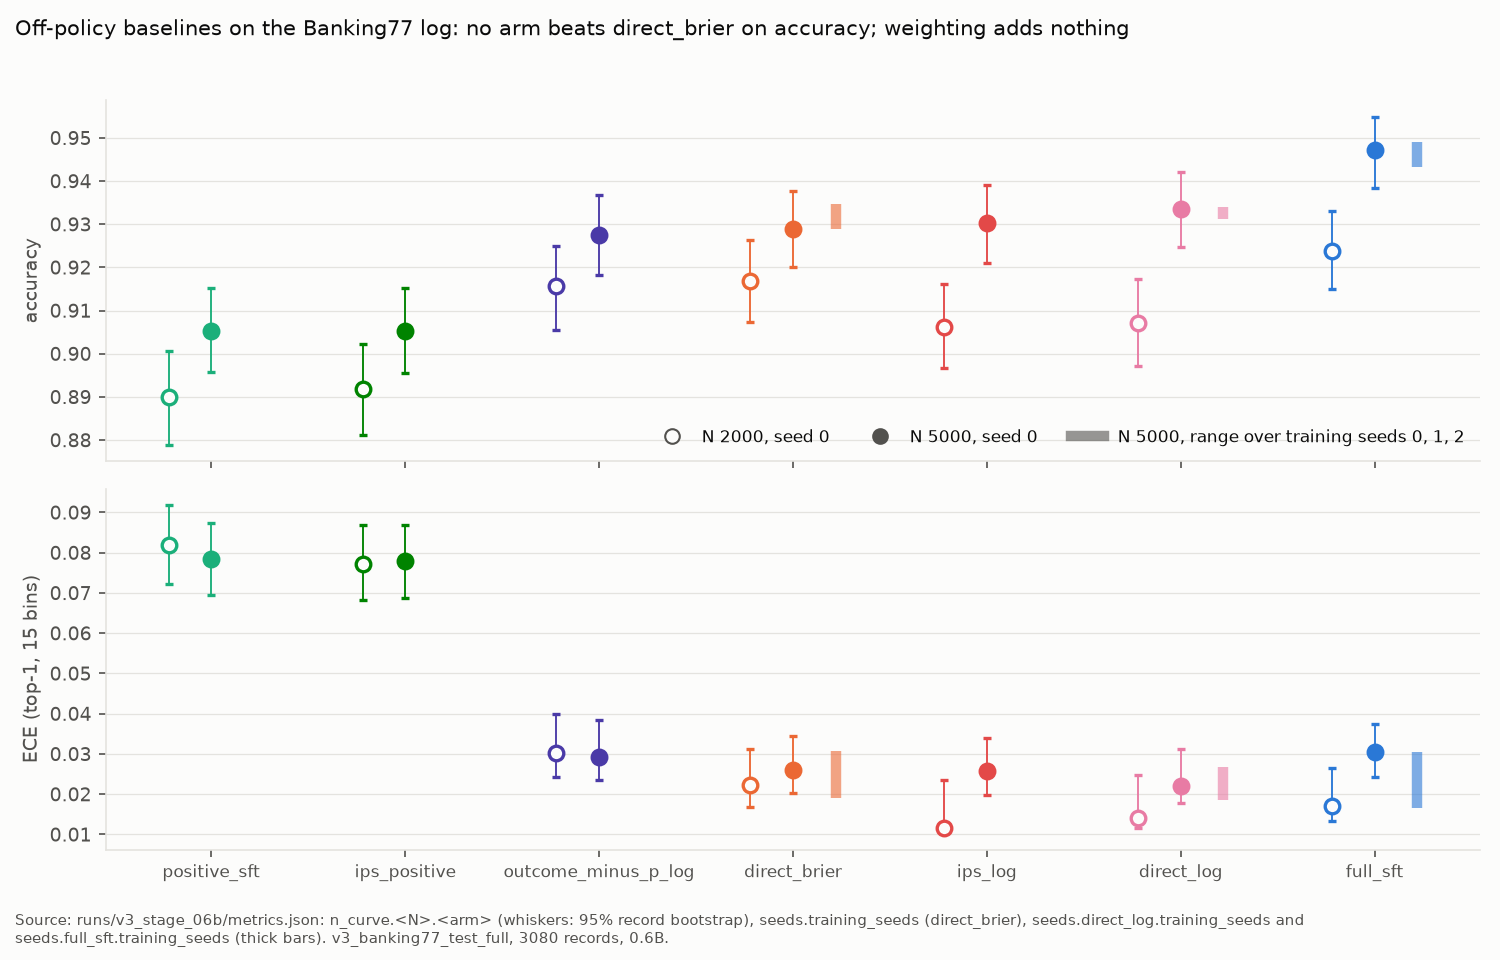
\includegraphics[width=\textwidth]{figures/v4_offpolicy.png}
\caption{Off-policy baselines on the Banking77 log at N 2000 and 5000, 0.6B: accuracy and ECE per arm, with the range over three training seeds at N 5000 where they exist. Provenance: Table~\ref{tab:prov}, F3.}\label{fig:v4_offpolicy}
\end{figure}

\subsection{Noise-rate sweep, N 5000, seed 0}\label{sec:A4}

\begin{table}[H]
\centering
\footnotesize
\setlength{\tabcolsep}{3pt}
\caption{Noise-rate sweep, N 5000, seed 0. ``Final step'' is step 1407, the end of the budget.}
\label{tab:A4}
\begin{adjustbox}{max width=\textwidth}
\begin{tabular}{llrrrrrrrr}
\toprule
f & learner & accuracy & minus clean & channel-scale ECE & reference & mean top-1 & channel line & final-step accuracy & criterion growth \\
\midrule
0 & CAPS-Brier & .929 &  &  &  &  &  & .933 & .059 \\
0.1 & CAPS-Brier & .923 [.914, .932] & $-$.006 [$-$.013, +.001] & .038 [.035, .046] & .021 & .870 & .838 & .892 & .114 \\
0.2 & CAPS-Brier & .907 [.897, .916] & $-$.022 [$-$.030, $-$.014] & .058 [.052, .063] & .014 & .743 & .744 & .813 & .284 \\
0.3 & CAPS-Brier & .888 [.877, .898] & $-$.041 [$-$.050, $-$.032] & .069 [.065, .073] & .009 & .674 & .655 & .734 & .757 \\
0 & \texttt{positive\_sft} & .905 &  &  &  &  &  &  & .268 \\
0.1 & \texttt{positive\_sft} & .890 [.880, .901] & $-$.015 [$-$.021, $-$.008] & .124 [.118, .133] & .063 & .935 & .812 &  & 1.244 \\
0.2 & \texttt{positive\_sft} & .866 [.855, .878] & $-$.039 [$-$.048, $-$.031] & .196 [.190, .203] & .047 & .915 & .720 &  & 2.216 \\
0.3 & \texttt{positive\_sft} & .867 [.856, .879] & $-$.038 [$-$.046, $-$.030] & .251 [.247, .256] & .031 & .896 & .647 &  & 2.916 \\
\bottomrule
\end{tabular}
\end{adjustbox}
\end{table}

CAPS-Brier's excess channel-scale ECE over a channel-calibrated copy of the clean run grows with f: .017, .044 and .060. Its accuracy loss against \texttt{positive\_sft}'s is +.009 [+.000, +.018] at 0.1 and +.017 [+.007, +.028] at 0.2. A soft-target diagnostic removes most of the residual; it needs the clean outcome, so it is a diagnostic, not a learner: channel-scale ECE .019 to .024 against a reference of .014 (R3, Section~4). The residual is therefore the variance of one noisy draw per interaction, not a limit of the objective.

\subsection{Scale: 1.7B against 0.6B at N 5000}\label{sec:A5}

\begin{table}[H]
\centering
\footnotesize
\setlength{\tabcolsep}{3pt}
\caption{Scale: 1.7B against 0.6B at N 5000. The 1.7B columns are seed 0; CAPS-Brier's three-seed row and differences follow the tables.}
\label{tab:A5}
\begin{adjustbox}{max width=\textwidth}
\begin{tabular}{llrrrrrrrr}
\toprule
learner & 1.7B accuracy & 1.7B ECE & 1.7B Brier & 1.7B NLL & 1.7B AURC & 1.7B Cov@.05 & 0.6B accuracy, seed 0 & 0.6B accuracy, seed mean (range) & 0.6B ECE, seed mean \\
\midrule
zero-shot & .848 [.836, .860] & .089 [.078, .100] & .242 & .660 & .0350 [.0301, .0401] & .731 [.699, .763] & .851 &  & .063 \\
temperature & .848 & .031 [.026, .044] & .222 & .519 & .0333 [.0285, .0382] & .750 [.719, .774] & .851 &  & .020 \\
\texttt{positive\_sft} & .913 [.902, .923] & .067 [.058, .077] & .154 & .545 & .0177 [.0139, .0218] & .906 [.877, .933] & .905 & (seed 0 only) & .078 \\
CAPS-Brier & .949 [.941, .957] & .021 [.015, .028] & .079 & .188 & .0066 [.0049, .0084] & .998 [.981, 1.000] & .929 & .931 (.929, .935) & .025 \\
\texttt{full\_sft} & .953 [.945, .960] & .023 [.018, .030] & .072 & .162 & .0053 [.0037, .0071] & 1.000 [.991, 1.000] & .947 & .946 (.943, .949) & .022 \\
\bottomrule
\end{tabular}
\end{adjustbox}
\end{table}

\begin{table}[H]
\centering
\footnotesize
\setlength{\tabcolsep}{3pt}
\caption{Scale: paired differences at 1.7B, N 5000.}
\label{tab:A5b}
\begin{adjustbox}{max width=\textwidth}
\begin{tabular}{llrrrrr}
\toprule
1.7B paired difference & accuracy & ECE & Brier & NLL & AURC & Cov@.05 \\
\midrule
CAPS-Brier seed 0 minus \texttt{positive\_sft} & +.036 [+.028, +.045] & $-$.046 [$-$.054, $-$.037] & $-$.075 [$-$.088, $-$.061] & $-$.357 [$-$.411, $-$.306] & $-$.0111 [$-$.0145, $-$.0083] & +.093 [+.065, +.115] \\
CAPS-Brier seed 0 minus \texttt{full\_sft} & $-$.004 [$-$.010, +.002] & $-$.002 [$-$.008, +.004] & +.007 [+.001, +.013] & +.026 [+.013, +.040] & +.0013 [+.0004, +.0022] & $-$.002 [$-$.015, +.001] \\
CAPS-Brier seed mean minus \texttt{positive\_sft} & +.034 [+.026, +.041] & $-$.051 [$-$.057, $-$.040] & $-$.070 [$-$.083, $-$.057] & $-$.353 [$-$.409, $-$.303] & $-$.0104 [$-$.0135, $-$.0078] & +.088 [+.062, +.108] \\
CAPS-Brier seed mean minus \texttt{full\_sft} & $-$.006 [$-$.011, $-$.002] & $-$.007 [$-$.011, +.000] & +.012 [+.006, +.017] & +.030 [+.018, +.043] & +.0021 [+.0012, +.0030] & $-$.0068 [$-$.0187, $-$.0002] \\
\bottomrule
\end{tabular}
\end{adjustbox}
\end{table}

CAPS-Brier at 1.7B over training seeds 0, 1 and 2, mean (range): accuracy .947 (.942, .949), ECE .016 (.013, .021), Brier .084 (.079, .093), NLL .192 (.182, .205), AURC .0073 (.0066, .0085), Cov@.05 .993 (.983, .998). The differences above put the seed mean against the single seed of each baseline. Every 1.7B CAPS-Brier seed is above every 0.6B one (.942 to .949 against .929 to .935).

\subsection{Full labels: unseen-schema ECE, 0.6B, three seeds}\label{sec:A6}

\begin{table}[H]
\centering
\small
\caption{Full labels: unseen-schema ECE, 0.6B, three seeds.}
\label{tab:A6}
\begin{adjustbox}{max width=\textwidth}
\begin{tabular}{llrr}
\toprule
run & unseen mean ECE (seeds 0, 1, 2) & minus SFT + T [95\% CI] & with its own temperature, minus SFT + T \\
\midrule
SFT & .152 &  &  \\
SFT + T & .121 &  &  \\
continued cross-entropy & .171 (.185, .172, .156) & +.050 [+.044, +.056] & +.002 [$-$.001, +.009] \\
REINFORCE, outcome & .248 (.262, .244, .239) & +.127 [+.118, +.135] & +.025 [+.018, +.034] \\
REINFORCE, $r - p$ & .153 (.173, .155, .131) & +.031 [+.026, +.038] & $-$.002 [$-$.006, +.004] \\
CAPS-Brier & .159 (.173, .165, .139) & +.037 [+.032, +.043] & +.001 [$-$.004, +.007] \\
CAPS-log & .170 (.181, .172, .156) & +.048 [+.043, +.055] & +.005 [+.001, +.011] \\
\bottomrule
\end{tabular}
\end{adjustbox}
\end{table}

\subsection{Emotion, 0.6B}\label{sec:A7}

AURC is lower for CAPS-Brier than for \texttt{positive\_sft} by .050 to .174, and at N 5000 its Cov@.05 is .595 against .032. \texttt{positive\_sft} trains on 206 to 2151 confirmed answers and is worse calibrated than zero-shot at every N (ECE .256 to .363 against .251). Against \texttt{full\_sft}, CAPS-Brier is 3.8 to 4.6 points below on seed 0 and closes 68, 79 and 88 percent of the accuracy gap between zero-shot (.540) and \texttt{full\_sft}, computed from the stored accuracies. Its seeds span accuracy .821 to .832 and ECE .031 to .070. CAPS-log at N 5000 is $-$.021 [$-$.030, $-$.012] below CAPS-Brier's seed mean in accuracy, with higher Brier and NLL, so Brier stays the default. The temperature learner (T about 2.3) has the lowest ECE, .024 at N 5000, and leaves AURC at .294 against zero-shot's .295: it fixes the level, not the ranking. At N 5000, CAPS-Brier costs 1.9 to 2.6 points of in-domain accuracy across seeds and \texttt{full\_sft} 3.4, both with in-domain ECE within .004 of zero-shot. The label audit finds a problem in .32 and .40 of a uniform sample, mostly a labelling convention that follows emotion words (.20), and no plainly wrong label; the ceiling is .93 or higher if the convention is learnable and near .80 if it is not, and \texttt{full\_sft} and every CAPS-Brier seed are above .80. On the 500-record emotion subset, gpt-4.1-mini scores .598 and CAPS-Brier at N 5000 .842 to .858, with no paired interval.


\begin{table}[H]
\centering
\footnotesize
\setlength{\tabcolsep}{3pt}
\caption{Emotion, 0.6B: the N-curve (CAPS-Brier seed 0). Brackets are 95 percent record-bootstrap intervals; AURC and Cov@.05 rank by top-1 probability.}
\label{tab:A7}
\begin{adjustbox}{max width=\textwidth}
\begin{tabular}{llrrrrr}
\toprule
N & metric & zero-shot & temperature & \texttt{positive\_sft} & \texttt{full\_sft} & CAPS-Brier \\
\midrule
500 & accuracy & .540 [.518, .562] & .540 & .578 [.555, .599] & .659 [.640, .681] & .621 [.601, .642] \\
2000 & accuracy & .540 & .540 & .589 [.567, .611] & .760 [.742, .779] & .715 [.695, .734] \\
5000 & accuracy & .540 & .540 & .615 [.592, .636] & .871 [.856, .884] & .832 [.816, .848] \\
500 & ECE & .251 [.232, .272] & .031 [.024, .056] & .363 [.342, .385] & .066 [.057, .091] & .087 [.075, .110] \\
2000 & ECE & .251 & .027 [.021, .053] & .324 [.304, .344] & .056 [.043, .075] & .066 [.049, .085] \\
5000 & ECE & .251 & .024 [.020, .051] & .256 [.237, .277] & .041 [.031, .055] & .070 [.059, .087] \\
500 & Brier & .687 [.657, .718] & .600 [.580, .620] & .764 [.724, .805] & .482 [.457, .505] & .534 [.509, .559] \\
2000 & Brier & .687 & .600 [.580, .620] & .708 [.671, .744] & .346 [.321, .369] & .422 [.399, .446] \\
5000 & Brier & .687 & .600 [.580, .619] & .628 [.593, .662] & .193 [.175, .213] & .264 [.241, .288] \\
500 & NLL & 1.675 [1.579, 1.759] & 1.251 [1.209, 1.292] & 3.147 [2.939, 3.327] & .980 [.927, 1.030] & 1.154 [1.094, 1.212] \\
2000 & NLL & 1.675 & 1.251 [1.209, 1.292] & 2.256 [2.111, 2.389] & .697 [.644, .750] & .877 [.830, .924] \\
5000 & NLL & 1.675 & 1.251 [1.210, 1.291] & 1.641 [1.532, 1.741] & .383 [.340, .428] & .599 [.541, .657] \\
500 & AURC & .295 [.272, .321] & .294 [.270, .320] & .262 [.236, .286] & .190 [.170, .209] & .212 [.193, .234] \\
2000 & AURC & .295 & .294 [.270, .320] & .254 [.231, .277] & .101 [.088, .115] & .148 [.130, .165] \\
5000 & AURC & .295 & .294 [.270, .320] & .233 [.211, .255] & .031 [.025, .037] & .058 [.048, .069] \\
500 & Cov@.05 & .025 [.007, .062] & .014 [.007, .055] & .002 [.001, .029] & .072 [.041, .118] & .068 [.024, .105] \\
2000 & Cov@.05 & .025 & .014 [.007, .055] & .030 [.011, .054] & .277 [.163, .389] & .107 [.065, .219] \\
5000 & Cov@.05 & .025 & .015 [.007, .055] & .032 [.005, .071] & .762 [.689, .813] & .595 [.470, .660] \\
\bottomrule
\end{tabular}
\end{adjustbox}
\end{table}

\begin{table}[H]
\centering
\footnotesize
\setlength{\tabcolsep}{3pt}
\caption{Emotion, 0.6B: paired differences, CAPS-Brier minus the other learner.}
\label{tab:A7b}
\begin{adjustbox}{max width=\textwidth}
\begin{tabular}{llrrrrrr}
\toprule
N & vs & accuracy & ECE & Brier & NLL & AURC & Cov@.05 \\
\midrule
500 & \texttt{positive\_sft} & +.043 [+.027, +.060] & $-$.276 [$-$.290, $-$.254] & $-$.230 [$-$.257, $-$.206] & $-$1.993 [$-$2.138, $-$1.841] & $-$.050 [$-$.064, $-$.036] & +.066 [+.019, +.101] \\
2000 & \texttt{positive\_sft} & +.126 [+.109, +.144] & $-$.258 [$-$.282, $-$.232] & $-$.286 [$-$.313, $-$.261] & $-$1.379 [$-$1.482, $-$1.273] & $-$.106 [$-$.121, $-$.093] & +.077 [+.036, +.182] \\
5000 & \texttt{positive\_sft} & +.217 [+.197, +.238] & $-$.186 [$-$.204, $-$.162] & $-$.364 [$-$.396, $-$.330] & $-$1.042 [$-$1.134, $-$.947] & $-$.174 [$-$.195, $-$.154] & +.564 [+.439, +.632] \\
500 & \texttt{full\_sft} & $-$.038 [$-$.053, $-$.025] & +.021 [+.001, +.037] & +.053 [+.041, +.064] & +.174 [+.146, +.204] & +.022 [+.014, +.030] & $-$.005 [$-$.035, +.025] \\
2000 & \texttt{full\_sft} & $-$.046 [$-$.060, $-$.033] & +.010 [$-$.009, +.027] & +.076 [+.066, +.087] & +.180 [+.154, +.206] & +.047 [+.039, +.054] & $-$.170 [$-$.242, $-$.030] \\
5000 & \texttt{full\_sft} & $-$.039 [$-$.052, $-$.027] & +.029 [+.017, +.043] & +.070 [+.056, +.088] & +.216 [+.178, +.261] & +.027 [+.020, +.035] & $-$.167 [$-$.260, $-$.100] \\
\bottomrule
\end{tabular}
\end{adjustbox}
\end{table}

\begin{table}[H]
\centering
\footnotesize
\setlength{\tabcolsep}{3pt}
\caption{Emotion, 0.6B: CAPS-Brier at N 5000 over training seeds.}
\label{tab:A7c}
\begin{adjustbox}{max width=\textwidth}
\begin{tabular}{llrrrrrrr}
\toprule
run & accuracy & ECE & Brier & NLL & AURC & Cov@.05 & minus seed 0, accuracy & minus seed 0, ECE \\
\midrule
seed 0 & .832 [.816, .848] & .070 [.059, .087] & .264 & .599 & .058 & .595 &  &  \\
seed 1 & .829 [.812, .845] & .031 [.024, .049] & .261 & .567 & .059 & .556 & $-$.003 [$-$.014, +.008] & $-$.039 [$-$.048, $-$.025] \\
seed 2 & .821 [.803, .837] & .038 [.028, .055] & .266 & .573 & .058 & .572 & $-$.011 [$-$.022, +.000] & $-$.032 [$-$.042, $-$.020] \\
mean of 3 training seeds (range) & .827 (.821, .832) & .046 (.031, .070) & .263 (.261, .266) & .580 (.567, .599) & .059 (.058, .059) & .575 (.556, .595) &  &  \\
\bottomrule
\end{tabular}
\end{adjustbox}
\end{table}

\begin{table}[H]
\centering
\footnotesize
\setlength{\tabcolsep}{3pt}
\caption{Emotion, 0.6B: CAPS-Brier seed mean minus the other learner, N 5000.}
\label{tab:A7d}
\begin{adjustbox}{max width=\textwidth}
\begin{tabular}{llrrrrr}
\toprule
seed mean minus & accuracy & ECE & Brier & NLL & AURC & Cov@.05 \\
\midrule
\texttt{positive\_sft} & +.213 [+.193, +.233] & $-$.210 [$-$.227, $-$.186] & $-$.364 [$-$.395, $-$.334] & $-$1.061 [$-$1.150, $-$.968] & $-$.174 [$-$.193, $-$.154] & +.543 [+.409, +.618] \\
\texttt{full\_sft} seed 0 & $-$.043 [$-$.056, $-$.031] & +.006 [$-$.005, +.018] & +.070 [+.056, +.085] & +.197 [+.164, +.235] & +.028 [+.022, +.034] & $-$.188 [$-$.297, $-$.128] \\
\bottomrule
\end{tabular}
\end{adjustbox}
\end{table}

\begin{table}[H]
\centering
\small
\caption{Emotion, 0.6B: forgetting at N 5000, minus zero-shot (\texttt{test\_indomain} .956, \texttt{test\_unseen\_intents} .892).}
\label{tab:A7e}
\begin{adjustbox}{max width=\textwidth}
\begin{tabular}{llrrr}
\toprule
run & \texttt{test\_indomain} accuracy & \texttt{test\_indomain} ECE & \texttt{test\_unseen\_intents} accuracy & \texttt{test\_unseen\_intents} ECE \\
\midrule
\texttt{positive\_sft} & $-$.005 [$-$.007, $-$.002] & +.007 [+.004, +.009] & +.010 [+.006, +.013] & $-$.003 [$-$.007, +.000] \\
CAPS-Brier seed 0 & $-$.026 [$-$.031, $-$.023] & +.001 [$-$.004, +.004] & $-$.020 [$-$.027, $-$.013] & +.002 [$-$.005, +.009] \\
CAPS-Brier seed 1 & $-$.019 [$-$.023, $-$.015] & +.003 [$-$.002, +.009] & $-$.024 [$-$.031, $-$.017] & $-$.017 [$-$.025, $-$.011] \\
CAPS-Brier seed 2 & $-$.024 [$-$.027, $-$.020] & $-$.003 [$-$.007, +.004] & $-$.034 [$-$.042, $-$.026] & +.000 [$-$.008, +.007] \\
CAPS-log & $-$.022 [$-$.026, $-$.019] & $-$.001 [$-$.006, +.003] & $-$.011 [$-$.018, $-$.004] & $-$.013 [$-$.020, $-$.007] \\
\texttt{full\_sft} & $-$.034 [$-$.038, $-$.029] & $-$.002 [$-$.007, +.001] & $-$.040 [$-$.048, $-$.032] & +.011 [+.003, +.018] \\
\bottomrule
\end{tabular}
\end{adjustbox}
\end{table}

\clearpage
\section{Setup and reproducibility details}\label{sec:setup}

\textbf{Model and training.} LoRA has r 16 and alpha 32 on the attention projections, and answers are read from the letter logits at each question's answer slot in one forward pass. Supervised training samples options per record, with negated yes-or-no phrasings. In adaptation, all trained learners take the same number of steps, $\max(200, \lceil 10 \times 0.9 N / 32 \rceil)$, at lr 5e-5, and bootstrap intervals use 1000 resamples over records, paired across runs.

\textbf{Group baselines.} \texttt{rlcd.normalize\_std: false} is set in \texttt{configs/rlcd\_06b.yaml} and in the \texttt{config.yaml} of all 31 full-label runs, so the full-label group baseline subtracts the group mean only; the logged-feedback REINFORCE arm subtracts the batch mean only.

\textbf{Learners.}
\begin{itemize}
  \item Temperature fitted to the logged outcomes: post-hoc and global, and it changes no argmax.
  \item \texttt{positive\_sft}: cross-entropy on confirmed actions, positive-unlabeled learning with the negatives discarded, not unobserved. What practitioners do.
  \item \texttt{full\_sft}: cross-entropy on gold for every logged interaction. The upper bound, at one label per interaction.
\end{itemize}

\textbf{Leak and duplicate gates.} Before any GPU run, the data must pass two CPU checks:
\begin{itemize}
  \item state-free leak probes: classifiers on phrasing, question text and structure, which must not beat chance by more than a fixed margin and a shuffled-target null;
  \item train-test duplicate rules.
\end{itemize}

The Banking77 log domain drops 30 messages that match the test split and 31 repeats.

\textbf{Off-policy forms}, all on the same log:
\begin{itemize}
  \item REINFORCE with reward $r - p_a$, detached, a batch-mean baseline and the importance weight $\min(p/q, 5)$ (\texttt{outcome\_minus\_p\_log});
  \item CAPS with the log score and inverse propensity weighting of the direct-method loss, $\min(1/q, 5)$ divided by its mean over the training prefix (\texttt{ips\_log}), which is importance-weighted regression;
  \item \texttt{positive\_sft} with the same weights (\texttt{ips\_positive}).
\end{itemize}

\textbf{Metrics.} AURC is the mean error of the kept answers over all coverages; Cov@eps is computed for eps in \{.05, .10, .20\}, with ties in top-1 kept or dropped together. Every trained learner reaches Cov@.20 = 1, and from N 2000 Cov@.10 = 1 as well, so the tables show Cov@.05. The same metrics ranked by the response's confidence field, $1 - H/\ln K$, are stored under \texttt{\_entropy} keys.

\textbf{Label audits.} Two language-model judges, no human, audited the labels. On Banking77 they find some label problem in .12 and .14 of a uniform sample and a clearly wrong label in .04, and a problem in .66 and .62 of 100 questions both \texttt{full\_sft} and CAPS-Brier miss, so the ceiling is plausibly near .96 (\texttt{docs/audit/SUMMARY.md}). On emotion they find a problem in .32 and .40 of a uniform sample, mostly a labelling convention that follows emotion words (.20 for both judges) (\texttt{docs/audit/EMOTION\_SUMMARY.md}).

\textbf{Commits of the runs:}
\begin{itemize}
  \item b5913ef: the v3 logs and the phase 3 runs;
  \item b6b9e85 and 409c983: the off-policy runs;
  \item 36e8ee1: the noise sweep;
  \item c9e29c6: the 1.7B runs;
  \item 344019b: the 1.7B CAPS-Brier seeds 1 and 2;
  \item c86d322: the emotion log and runs;
  \item b9c0257: AURC and Cov@eps added to every run and stage file, earlier values unchanged.
\end{itemize}

{\sloppy \textbf{Tables and figures:} every table is regenerated on CPU from committed files by \texttt{scripts/compare\_v3.py}, \texttt{scripts/compare\_noise.py}, \texttt{scripts/compare\_rlcd.py}, \texttt{scripts/paired\_deltas.py} and \texttt{scripts/log\_stats.py}. Every figure is regenerated by \texttt{scripts/make\_figures.py}. The training scripts (\texttt{scripts/train\_sft.py}, \texttt{scripts/train\_rlcd.py}) fit one Kaggle T4 session per run (\texttt{docs/KAGGLE.md}).\par}

\clearpage
\section{Provenance}\label{sec:B}
\counterwithout{table}{subsection}
\counterwithin{table}{section}

Every number in the paper comes from a committed file in the repository at the commits listed in Section~\ref{sec:7}. Table~\ref{tab:prov} gives, for each table (T), figure (F) and in-text result (S), the file and the keys within it; \texttt{<N>}, \texttt{<f>}, \texttt{<learner>}, \texttt{<arm>}, \texttt{<split>}, \texttt{<k>} and \texttt{<run>} stand for the log size, flip rate, learner, arm, evaluation split, training seed and run directory. R1, R2 and R3 are the project reports \texttt{docs/RESULTS\_v1.md}, \texttt{RESULTS\_v2.md} and \texttt{RESULTS\_v3.md}, and the report column gives the section with the full analysis.

{\footnotesize
\setlength{\tabcolsep}{4pt}
\begin{longtable}{@{}p{0.05\textwidth}>{\raggedright\arraybackslash}p{0.24\textwidth}>{\raggedright\arraybackslash}p{0.53\textwidth}>{\raggedright\arraybackslash}p{0.11\textwidth}@{}}
\caption{Provenance of every table, figure and in-text result.}\label{tab:prov}\\
\toprule
No. & Item & File: keys & Report \\
\midrule
\endfirsthead
\toprule
No. & Item & File: keys & Report \\
\midrule
\endhead
\bottomrule
\endfoot
T1 & Table~\ref{tab:A1}, N-curve & \texttt{runs/\allowbreak{}v3\_\allowbreak{}stage\_\allowbreak{}06b/\allowbreak{}metrics.\allowbreak{}json}: \texttt{n\_\allowbreak{}curve.\allowbreak{}\textless{}N\textgreater{}.\allowbreak{}\textless{}learner\textgreater{};\allowbreak{} n\_\allowbreak{}curve.\allowbreak{}\textless{}N\textgreater{}.\allowbreak{}\textless{}learner\textgreater{}.\allowbreak{}coverage\_\allowbreak{}at\_\allowbreak{}\{0.\allowbreak{}10,0.\allowbreak{}20\}} & R3 \S2 \\
T2 & Table~\ref{tab:A1b}, N-curve differences & \texttt{runs/\allowbreak{}v3\_\allowbreak{}stage\_\allowbreak{}06b/\allowbreak{}metrics.\allowbreak{}json}: \texttt{n\_\allowbreak{}curve.\allowbreak{}\textless{}N\textgreater{}.\allowbreak{}direct\_\allowbreak{}brier\_\allowbreak{}minus\_\allowbreak{}\{positive\_\allowbreak{}sft,full\_\allowbreak{}sft\}} & R3 \S2 \\
T3 & Table~\ref{tab:A2}, training seeds & \texttt{runs/\allowbreak{}v3\_\allowbreak{}stage\_\allowbreak{}06b/\allowbreak{}metrics.\allowbreak{}json}: \texttt{seeds.\allowbreak{}training\_\allowbreak{}seeds;\allowbreak{} seeds.\allowbreak{}direct\_\allowbreak{}log.\allowbreak{}training\_\allowbreak{}seeds;\allowbreak{} seeds.\allowbreak{}full\_\allowbreak{}sft.\allowbreak{}training\_\allowbreak{}seeds} & R3 \S\S3, 11 \\
T4 & Table~\ref{tab:A2b}, seed-mean differences & \texttt{runs/\allowbreak{}v3\_\allowbreak{}stage\_\allowbreak{}06b/\allowbreak{}metrics.\allowbreak{}json}: \texttt{seeds.\allowbreak{}training\_\allowbreak{}seed\_\allowbreak{}mean\_\allowbreak{}minus\_\allowbreak{}positive\_\allowbreak{}sft;\allowbreak{} seeds.\allowbreak{}training\_\allowbreak{}seed\_\allowbreak{}mean\_\allowbreak{}minus\_\allowbreak{}full\_\allowbreak{}sft\_\allowbreak{}seed\_\allowbreak{}mean;\allowbreak{} seeds.\allowbreak{}direct\_\allowbreak{}log\_\allowbreak{}seed\_\allowbreak{}mean\_\allowbreak{}minus\_\allowbreak{}direct\_\allowbreak{}brier\_\allowbreak{}seed\_\allowbreak{}mean} & R3 \S\S3, 11 \\
T5 & Table~\ref{tab:A3}, off-policy baselines & \texttt{runs/\allowbreak{}v3\_\allowbreak{}stage\_\allowbreak{}06b/\allowbreak{}metrics.\allowbreak{}json}: \texttt{n\_\allowbreak{}curve.\allowbreak{}\textless{}N\textgreater{}.\allowbreak{}\textless{}arm\textgreater{};\allowbreak{} n\_\allowbreak{}curve.\allowbreak{}\textless{}N\textgreater{}.\allowbreak{}off\_\allowbreak{}policy.\allowbreak{}\textless{}arm\textgreater{}.\allowbreak{}minus\_\allowbreak{}direct\_\allowbreak{}brier} & R3 \S11 \\
T6 & Table~\ref{tab:A4}, noise-rate sweep & \texttt{runs/\allowbreak{}v3\_\allowbreak{}noise\_\allowbreak{}sweep\_\allowbreak{}06b/\allowbreak{}metrics.\allowbreak{}json}: \texttt{by\_\allowbreak{}rate.\allowbreak{}\textless{}f\textgreater{}.\allowbreak{}\textless{}arm\textgreater{};\allowbreak{} clean.\allowbreak{}\textless{}arm\textgreater{}} & R3 \S4 \\
T7 & Table~\ref{tab:A5}, scale & \texttt{runs/\allowbreak{}v3\_\allowbreak{}stage\_\allowbreak{}17b/\allowbreak{}metrics.\allowbreak{}json}: \texttt{n\_\allowbreak{}curve.\allowbreak{}5000.\allowbreak{}\textless{}learner\textgreater{}} \newline \texttt{runs/\allowbreak{}v3\_\allowbreak{}stage\_\allowbreak{}06b/\allowbreak{}metrics.\allowbreak{}json}: \texttt{n\_\allowbreak{}curve.\allowbreak{}5000.\allowbreak{}\textless{}learner\textgreater{};\allowbreak{} seeds.\allowbreak{}training\_\allowbreak{}seeds;\allowbreak{} seeds.\allowbreak{}full\_\allowbreak{}sft.\allowbreak{}training\_\allowbreak{}seeds} & R3 \S12 \\
T8 & Table~\ref{tab:A5b} and the three-seed values after it & \texttt{runs/\allowbreak{}v3\_\allowbreak{}stage\_\allowbreak{}17b/\allowbreak{}metrics.\allowbreak{}json}: \texttt{n\_\allowbreak{}curve.\allowbreak{}5000.\allowbreak{}direct\_\allowbreak{}brier\_\allowbreak{}minus\_\allowbreak{}\{positive\_\allowbreak{}sft,full\_\allowbreak{}sft\};\allowbreak{} seeds.\allowbreak{}training\_\allowbreak{}seeds;\allowbreak{} seeds.\allowbreak{}training\_\allowbreak{}seed\_\allowbreak{}mean\_\allowbreak{}minus\_\allowbreak{}\{positive\_\allowbreak{}sft,full\_\allowbreak{}sft\}} & R3 \S12 \\
T9 & Table~\ref{tab:A6}, full labels & \texttt{runs/\allowbreak{}rlcd\_\allowbreak{}stage2a\_\allowbreak{}06b/\allowbreak{}metrics.\allowbreak{}json}: \texttt{unseen\_\allowbreak{}schemas;\allowbreak{} temperature\_\allowbreak{}ablation} & R2 \S3 \\
T10 & Table~\ref{tab:A7}, emotion N-curve & \texttt{runs/\allowbreak{}v3\_\allowbreak{}stage\_\allowbreak{}emotion\_\allowbreak{}06b/\allowbreak{}metrics.\allowbreak{}json}: \texttt{n\_\allowbreak{}curve.\allowbreak{}\textless{}N\textgreater{}.\allowbreak{}\textless{}learner\textgreater{}} & R3 \S13 \\
T11 & Table~\ref{tab:A7b}, emotion differences & \texttt{runs/\allowbreak{}v3\_\allowbreak{}stage\_\allowbreak{}emotion\_\allowbreak{}06b/\allowbreak{}metrics.\allowbreak{}json}: \texttt{n\_\allowbreak{}curve.\allowbreak{}\textless{}N\textgreater{}.\allowbreak{}direct\_\allowbreak{}brier\_\allowbreak{}minus\_\allowbreak{}\{positive\_\allowbreak{}sft,full\_\allowbreak{}sft\}} & R3 \S13 \\
T12 & Table~\ref{tab:A7c}, emotion seeds & \texttt{runs/\allowbreak{}v3\_\allowbreak{}stage\_\allowbreak{}emotion\_\allowbreak{}06b/\allowbreak{}metrics.\allowbreak{}json}: \texttt{seeds.\allowbreak{}seed\_\allowbreak{}\textless{}k\textgreater{};\allowbreak{} seeds.\allowbreak{}minus\_\allowbreak{}seed\_\allowbreak{}0;\allowbreak{} seeds.\allowbreak{}training\_\allowbreak{}seeds} & R3 \S13 \\
T13 & Table~\ref{tab:A7d}, emotion seed-mean differences & \texttt{runs/\allowbreak{}v3\_\allowbreak{}stage\_\allowbreak{}emotion\_\allowbreak{}06b/\allowbreak{}metrics.\allowbreak{}json}: \texttt{seeds.\allowbreak{}training\_\allowbreak{}seed\_\allowbreak{}mean\_\allowbreak{}minus\_\allowbreak{}\{positive\_\allowbreak{}sft,full\_\allowbreak{}sft\}} & R3 \S13 \\
T14 & Table~\ref{tab:A7e}, emotion forgetting & \texttt{runs/\allowbreak{}v3\_\allowbreak{}stage\_\allowbreak{}emotion\_\allowbreak{}06b/\allowbreak{}metrics.\allowbreak{}json}: \texttt{forgetting.\allowbreak{}\textless{}split\textgreater{}.\allowbreak{}minus\_\allowbreak{}zero\_\allowbreak{}shot} & R3 \S13 \\
F1 & Figure~\ref{fig:v2_arm_ece} & \texttt{runs/\allowbreak{}rlcd\_\allowbreak{}stage2a\_\allowbreak{}06b/\allowbreak{}metrics.\allowbreak{}json}: \texttt{unseen\_\allowbreak{}schemas;\allowbreak{} temperature\_\allowbreak{}ablation} \newline \texttt{runs/\allowbreak{}rlcd\_\allowbreak{}06b\_\allowbreak{}\textless{}arm\textgreater{}\_\allowbreak{}s\textless{}k\textgreater{}\_\allowbreak{}temp/\allowbreak{}metrics.\allowbreak{}json}: \texttt{per-seed values after temperature} & R2 \S3 \\
F2 & Figure~\ref{fig:v3_n_curve} & \texttt{runs/\allowbreak{}v3\_\allowbreak{}stage\_\allowbreak{}06b/\allowbreak{}metrics.\allowbreak{}json}: \texttt{n\_\allowbreak{}curve.\allowbreak{}\textless{}N\textgreater{}.\allowbreak{}\textless{}learner\textgreater{};\allowbreak{} seeds.\allowbreak{}training\_\allowbreak{}seeds;\allowbreak{} seeds.\allowbreak{}full\_\allowbreak{}sft.\allowbreak{}training\_\allowbreak{}seeds} & R3 \S\S2, 3 \\
F3 & Figure~\ref{fig:v4_offpolicy} & \texttt{runs/\allowbreak{}v3\_\allowbreak{}stage\_\allowbreak{}06b/\allowbreak{}metrics.\allowbreak{}json}: \texttt{n\_\allowbreak{}curve.\allowbreak{}\textless{}N\textgreater{}.\allowbreak{}\textless{}arm\textgreater{};\allowbreak{} seeds.\allowbreak{}training\_\allowbreak{}seeds;\allowbreak{} seeds.\allowbreak{}direct\_\allowbreak{}log.\allowbreak{}training\_\allowbreak{}seeds;\allowbreak{} seeds.\allowbreak{}full\_\allowbreak{}sft.\allowbreak{}training\_\allowbreak{}seeds} & R3 \S11 \\
F4 & Figure~\ref{fig:v4_noise_sweep} & \texttt{runs/\allowbreak{}v3\_\allowbreak{}noise\_\allowbreak{}sweep\_\allowbreak{}06b/\allowbreak{}metrics.\allowbreak{}json}: \texttt{clean.\allowbreak{}\textless{}arm\textgreater{};\allowbreak{} by\_\allowbreak{}rate.\allowbreak{}\textless{}f\textgreater{}.\allowbreak{}\textless{}arm\textgreater{} (accuracy, minus\_\allowbreak{}clean, channel.\allowbreak{}channel\_\allowbreak{}scale, selection, last)} \newline \texttt{runs/\allowbreak{}\textless{}run\textgreater{}\_\allowbreak{}inverted/\allowbreak{}metrics.\allowbreak{}json}: \texttt{stored\_\allowbreak{}channel} & R3 \S4 \\
F5 & Figure~\ref{fig:v4_scale} & \texttt{runs/\allowbreak{}v3\_\allowbreak{}stage\_\allowbreak{}06b/\allowbreak{}metrics.\allowbreak{}json}: \texttt{n\_\allowbreak{}curve.\allowbreak{}5000.\allowbreak{}\textless{}learner\textgreater{};\allowbreak{} seeds.\allowbreak{}training\_\allowbreak{}seeds;\allowbreak{} seeds.\allowbreak{}full\_\allowbreak{}sft.\allowbreak{}training\_\allowbreak{}seeds;\allowbreak{} forgetting.\allowbreak{}test\_\allowbreak{}indomain.\allowbreak{}minus\_\allowbreak{}zero\_\allowbreak{}shot} \newline \texttt{runs/\allowbreak{}v3\_\allowbreak{}stage\_\allowbreak{}17b/\allowbreak{}metrics.\allowbreak{}json}: \texttt{the same keys} & R3 \S12 \\
F6 & Figure~\ref{fig:v4_emotion_n_curve} & \texttt{runs/\allowbreak{}v3\_\allowbreak{}stage\_\allowbreak{}emotion\_\allowbreak{}06b/\allowbreak{}metrics.\allowbreak{}json}: \texttt{n\_\allowbreak{}curve.\allowbreak{}\textless{}N\textgreater{}.\allowbreak{}\textless{}learner\textgreater{};\allowbreak{} n\_\allowbreak{}curve.\allowbreak{}5000.\allowbreak{}direct\_\allowbreak{}log;\allowbreak{} seeds.\allowbreak{}training\_\allowbreak{}seeds} & R3 \S13 \\
S1 & Section~\ref{sec:1}: in-domain ECE .013 to .015, up to .22 off-domain & \texttt{runs/\allowbreak{}sft\_\allowbreak{}\{06b,17b\}/\allowbreak{}metrics.\allowbreak{}json}: \texttt{splits.\allowbreak{}\textless{}split\textgreater{}.\allowbreak{}overall.\allowbreak{}ece} & R1 \S2 \\
S2 & Sections~\ref{sec:1} and~\ref{sec:5}: the gap to full labels does not shrink with N & \texttt{runs/\allowbreak{}v3\_\allowbreak{}stage\_\allowbreak{}06b/\allowbreak{}metrics.\allowbreak{}json}: \texttt{n\_\allowbreak{}curve.\allowbreak{}\textless{}N\textgreater{}.\allowbreak{}direct\_\allowbreak{}brier\_\allowbreak{}minus\_\allowbreak{}full\_\allowbreak{}sft} & R3 \S8 \\
S3 & Section~\ref{sec:3}: logging policy, negatives off the top choice & \texttt{runs/\allowbreak{}v3\_\allowbreak{}log\_\allowbreak{}s0/\allowbreak{}metrics.\allowbreak{}json}: \texttt{negatives} & R3 \S1; METHOD \S2 \\
S4 & Section~\ref{sec:3} and Appendix~\ref{sec:setup}: mean-only group baseline & \texttt{configs/\allowbreak{}rlcd\_\allowbreak{}06b.\allowbreak{}yaml;\allowbreak{} runs/\allowbreak{}rlcd\_\allowbreak{}06b\_\allowbreak{}*/\allowbreak{}config.\allowbreak{}yaml}: \texttt{rlcd.\allowbreak{}normalize\_\allowbreak{}std} & R2 \S2 \\
S5 & Appendix~\ref{sec:setup}: log-domain duplicates & \texttt{data/\allowbreak{}v3\_\allowbreak{}manifest.\allowbreak{}json} & R3 \S1 \\
S6 & Section~\ref{sec:4.1}: policy accuracy and outcome rate & \texttt{runs/\allowbreak{}v3\_\allowbreak{}log\_\allowbreak{}s0/\allowbreak{}metrics.\allowbreak{}json}: \texttt{accuracy;\allowbreak{} outcome\_\allowbreak{}rate} & R3 \S1 \\
S7 & Section~\ref{sec:4.1} and Appendix~\ref{sec:A1}: temperature against AURC and Cov@.05 & \texttt{runs/\allowbreak{}v3\_\allowbreak{}stage\_\allowbreak{}06b/\allowbreak{}metrics.\allowbreak{}json}: \texttt{n\_\allowbreak{}curve.\allowbreak{}5000.\allowbreak{}\{zero\_\allowbreak{}shot,temperature\};\allowbreak{} n\_\allowbreak{}curve.\allowbreak{}5000.\allowbreak{}direct\_\allowbreak{}brier\_\allowbreak{}temp\_\allowbreak{}minus\_\allowbreak{}direct\_\allowbreak{}brier.\allowbreak{}aurc} & R3 \S2 \\
S8 & Section~\ref{sec:4.2}: the broken reward & \texttt{runs/\allowbreak{}sft\_\allowbreak{}06b/\allowbreak{}metrics.\allowbreak{}json;\allowbreak{} runs/\allowbreak{}rlcd\_\allowbreak{}06b\_\allowbreak{}brier\_\allowbreak{}s0/\allowbreak{}metrics.\allowbreak{}json}: \texttt{splits.\allowbreak{}\textless{}split\textgreater{}.\allowbreak{}score.\allowbreak{}accuracy} \newline \texttt{runs/\allowbreak{}rlcd\_\allowbreak{}06b\_\allowbreak{}brier\_\allowbreak{}s0/\allowbreak{}config.\allowbreak{}yaml}: \texttt{rlcd.\allowbreak{}normalize\_\allowbreak{}std} \newline \texttt{runs/\allowbreak{}advantage\_\allowbreak{}simulation\_\allowbreak{}06b/\allowbreak{}metrics.\allowbreak{}json}: \texttt{rewards} & R2 \S2 \\
S9 & Section~\ref{sec:4.2}: no gain on full labels & \texttt{runs/\allowbreak{}rlcd\_\allowbreak{}stage2a\_\allowbreak{}06b/\allowbreak{}metrics.\allowbreak{}json}: \texttt{unseen\_\allowbreak{}schemas.\allowbreak{}mean\_\allowbreak{}ece.\allowbreak{}sft\_\allowbreak{}temp;\allowbreak{} unseen\_\allowbreak{}schemas.\allowbreak{}arms.\allowbreak{}\textless{}arm\textgreater{};\allowbreak{} temperature\_\allowbreak{}ablation.\allowbreak{}arms.\allowbreak{}\textless{}arm\textgreater{}} & R2 \S3 \\
S10 & Section~\ref{sec:4.3} and Appendix~\ref{sec:A1}: the N-curve & \texttt{runs/\allowbreak{}v3\_\allowbreak{}stage\_\allowbreak{}06b/\allowbreak{}metrics.\allowbreak{}json}: \texttt{n\_\allowbreak{}curve.\allowbreak{}\textless{}N\textgreater{}.\allowbreak{}direct\_\allowbreak{}brier\_\allowbreak{}minus\_\allowbreak{}\{positive\_\allowbreak{}sft,full\_\allowbreak{}sft\};\allowbreak{} n\_\allowbreak{}curve.\allowbreak{}\textless{}N\textgreater{}.\allowbreak{}\textless{}learner\textgreater{}.\allowbreak{}accuracy;\allowbreak{} n\_\allowbreak{}curve.\allowbreak{}\textless{}N\textgreater{}.\allowbreak{}temperature} & R3 \S2 \\
S11 & Section~\ref{sec:4.3} and Appendix~\ref{sec:A2}: seeds & \texttt{runs/\allowbreak{}v3\_\allowbreak{}stage\_\allowbreak{}06b/\allowbreak{}metrics.\allowbreak{}json}: \texttt{seeds;\allowbreak{} direct\_\allowbreak{}brier\_\allowbreak{}temperatures} & R3 \S3 \\
S12 & Section~\ref{sec:4.3} and Appendix~\ref{sec:A3}: off-policy baselines & \texttt{runs/\allowbreak{}v3\_\allowbreak{}stage\_\allowbreak{}06b/\allowbreak{}metrics.\allowbreak{}json}: \texttt{n\_\allowbreak{}curve.\allowbreak{}\textless{}N\textgreater{}.\allowbreak{}off\_\allowbreak{}policy.\allowbreak{}ips\_\allowbreak{}positive.\allowbreak{}minus\_\allowbreak{}positive\_\allowbreak{}sft;\allowbreak{} seeds.\allowbreak{}direct\_\allowbreak{}log\_\allowbreak{}seed\_\allowbreak{}mean\_\allowbreak{}minus\_\allowbreak{}direct\_\allowbreak{}brier\_\allowbreak{}seed\_\allowbreak{}mean} \newline \texttt{runs/\allowbreak{}v3\_\allowbreak{}06b\_\allowbreak{}ips\_\allowbreak{}positive\_\allowbreak{}n5000\_\allowbreak{}s0/\allowbreak{}train\_\allowbreak{}summary.\allowbreak{}json}: \texttt{ips} & R3 \S11 \\
S13 & Section~\ref{sec:4.3} and Appendix~\ref{sec:A4}: noisy feedback & \texttt{runs/\allowbreak{}v3\_\allowbreak{}noise\_\allowbreak{}sweep\_\allowbreak{}06b/\allowbreak{}metrics.\allowbreak{}json}: \texttt{by\_\allowbreak{}rate.\allowbreak{}\textless{}f\textgreater{}.\allowbreak{}direct\_\allowbreak{}brier.\allowbreak{}channel.\allowbreak{}channel\_\allowbreak{}scale.\allowbreak{}channel\_\allowbreak{}ece\_\allowbreak{}minus\_\allowbreak{}reference;\allowbreak{} by\_\allowbreak{}rate.\allowbreak{}\textless{}f\textgreater{}.\allowbreak{}direct\_\allowbreak{}brier.\allowbreak{}channel.\allowbreak{}inverted\_\allowbreak{}top1\_\allowbreak{}ece;\allowbreak{} by\_\allowbreak{}rate.\allowbreak{}\textless{}f\textgreater{}.\allowbreak{}amplification;\allowbreak{} clean.\allowbreak{}direct\_\allowbreak{}brier.\allowbreak{}ece;\allowbreak{} by\_\allowbreak{}rate.\allowbreak{}\textless{}f\textgreater{}.\allowbreak{}direct\_\allowbreak{}brier\_\allowbreak{}loss\_\allowbreak{}minus\_\allowbreak{}positive\_\allowbreak{}sft\_\allowbreak{}loss.\allowbreak{}accuracy;\allowbreak{} by\_\allowbreak{}rate.\allowbreak{}0.\allowbreak{}3.\allowbreak{}direct\_\allowbreak{}brier.\allowbreak{}last.\allowbreak{}accuracy;\allowbreak{} zero\_\allowbreak{}shot.\allowbreak{}accuracy;\allowbreak{} by\_\allowbreak{}rate.\allowbreak{}\textless{}f\textgreater{}.\allowbreak{}direct\_\allowbreak{}brier.\allowbreak{}selection.\allowbreak{}best\_\allowbreak{}step} & R3 \S4 \\
S14 & Section~\ref{sec:4.3} and Appendix~\ref{sec:A5}: scale & \texttt{runs/\allowbreak{}v3\_\allowbreak{}stage\_\allowbreak{}17b/\allowbreak{}metrics.\allowbreak{}json}: \texttt{seeds.\allowbreak{}training\_\allowbreak{}seeds;\allowbreak{} seeds.\allowbreak{}training\_\allowbreak{}seed\_\allowbreak{}mean\_\allowbreak{}minus\_\allowbreak{}\{positive\_\allowbreak{}sft,full\_\allowbreak{}sft\};\allowbreak{} n\_\allowbreak{}curve.\allowbreak{}5000.\allowbreak{}direct\_\allowbreak{}brier\_\allowbreak{}minus\_\allowbreak{}full\_\allowbreak{}sft} \newline \texttt{runs/\allowbreak{}v3\_\allowbreak{}stage\_\allowbreak{}06b/\allowbreak{}metrics.\allowbreak{}json}: \texttt{seeds.\allowbreak{}training\_\allowbreak{}seed\_\allowbreak{}mean\_\allowbreak{}minus\_\allowbreak{}full\_\allowbreak{}sft\_\allowbreak{}seed\_\allowbreak{}mean} & R3 \S12 \\
S15 & Section~\ref{sec:4.3}: forgetting and selective prediction & \texttt{runs/\allowbreak{}v3\_\allowbreak{}stage\_\allowbreak{}06b/\allowbreak{}metrics.\allowbreak{}json}: \texttt{forgetting;\allowbreak{} coverage.\allowbreak{}\{positive\_\allowbreak{}sft,direct\_\allowbreak{}brier\}\_\allowbreak{}n5000\_\allowbreak{}s0.\allowbreak{}0.\allowbreak{}95;\allowbreak{} n\_\allowbreak{}curve.\allowbreak{}5000.\allowbreak{}\{direct\_\allowbreak{}brier,positive\_\allowbreak{}sft\}.\allowbreak{}coverage\_\allowbreak{}at\_\allowbreak{}0.\allowbreak{}05} & R3 \S\S5, 6 \\
S16 & Section~\ref{sec:4.3}: against an API model & \texttt{runs/\allowbreak{}v3\_\allowbreak{}stage\_\allowbreak{}06b/\allowbreak{}metrics.\allowbreak{}json}: \texttt{b2\_\allowbreak{}reference} & R3 \S7 \\
S17 & Section~\ref{sec:4.4}: the emotion log & \texttt{runs/\allowbreak{}v3\_\allowbreak{}log\_\allowbreak{}emotion\_\allowbreak{}s0/\allowbreak{}metrics.\allowbreak{}json}: \texttt{accuracy;\allowbreak{} negatives.\allowbreak{}negatives} \newline \texttt{runs/\allowbreak{}v3\_\allowbreak{}log\_\allowbreak{}s0/\allowbreak{}metrics.\allowbreak{}json}: \texttt{outcome\_\allowbreak{}rate} & R3 \S13 \\
S18 & Section~\ref{sec:4.4} and Appendix~\ref{sec:A7}: emotion results & \texttt{runs/\allowbreak{}v3\_\allowbreak{}stage\_\allowbreak{}emotion\_\allowbreak{}06b/\allowbreak{}metrics.\allowbreak{}json}: \texttt{n\_\allowbreak{}curve.\allowbreak{}\textless{}N\textgreater{}.\allowbreak{}direct\_\allowbreak{}brier\_\allowbreak{}minus\_\allowbreak{}\{positive\_\allowbreak{}sft,full\_\allowbreak{}sft\};\allowbreak{} n\_\allowbreak{}curve.\allowbreak{}\textless{}N\textgreater{}.\allowbreak{}\textless{}learner\textgreater{};\allowbreak{} seeds.\allowbreak{}training\_\allowbreak{}seeds;\allowbreak{} seeds.\allowbreak{}training\_\allowbreak{}seed\_\allowbreak{}mean\_\allowbreak{}minus\_\allowbreak{}full\_\allowbreak{}sft;\allowbreak{} seeds.\allowbreak{}direct\_\allowbreak{}log\_\allowbreak{}seed\_\allowbreak{}mean\_\allowbreak{}minus\_\allowbreak{}direct\_\allowbreak{}brier\_\allowbreak{}seed\_\allowbreak{}mean;\allowbreak{} forgetting.\allowbreak{}test\_\allowbreak{}indomain.\allowbreak{}minus\_\allowbreak{}zero\_\allowbreak{}shot;\allowbreak{} b2\_\allowbreak{}reference} \newline \texttt{runs/\allowbreak{}v3\_\allowbreak{}emotion\_\allowbreak{}06b\_\allowbreak{}positive\_\allowbreak{}sft\_\allowbreak{}n\textless{}N\textgreater{}\_\allowbreak{}s0/\allowbreak{}train\_\allowbreak{}summary.\allowbreak{}json}: \texttt{n\_\allowbreak{}used} \newline \texttt{docs/\allowbreak{}audit/\allowbreak{}emotion\_\allowbreak{}summary.\allowbreak{}json}: \texttt{groups} & R3 \S13 \\
S19 & Section~\ref{sec:4.4}: the predictions & \texttt{runs/\allowbreak{}v3\_\allowbreak{}stage\_\allowbreak{}emotion\_\allowbreak{}06b/\allowbreak{}metrics.\allowbreak{}json}: \texttt{n\_\allowbreak{}curve.\allowbreak{}5000.\allowbreak{}direct\_\allowbreak{}brier\_\allowbreak{}minus\_\allowbreak{}full\_\allowbreak{}sft;\allowbreak{} seeds.\allowbreak{}training\_\allowbreak{}seed\_\allowbreak{}mean\_\allowbreak{}minus\_\allowbreak{}full\_\allowbreak{}sft} \newline \texttt{runs/\allowbreak{}v3\_\allowbreak{}stage\_\allowbreak{}06b/\allowbreak{}metrics.\allowbreak{}json}: \texttt{n\_\allowbreak{}curve.\allowbreak{}5000.\allowbreak{}direct\_\allowbreak{}brier\_\allowbreak{}minus\_\allowbreak{}full\_\allowbreak{}sft;\allowbreak{} seeds.\allowbreak{}training\_\allowbreak{}seed\_\allowbreak{}mean\_\allowbreak{}minus\_\allowbreak{}full\_\allowbreak{}sft\_\allowbreak{}seed\_\allowbreak{}mean} & R3 \S13 \\
S20 & Section~\ref{sec:5}: in-domain ECE of the noisy run & \texttt{runs/\allowbreak{}v3\_\allowbreak{}stage\_\allowbreak{}06b/\allowbreak{}metrics.\allowbreak{}json}: \texttt{forgetting.\allowbreak{}test\_\allowbreak{}indomain.\allowbreak{}minus\_\allowbreak{}zero\_\allowbreak{}shot.\allowbreak{}direct\_\allowbreak{}brier\_\allowbreak{}n5000\_\allowbreak{}s0\_\allowbreak{}noisy.\allowbreak{}ece} & R3 \S5 \\
S21 & Section~\ref{sec:5} and Appendix~\ref{sec:setup}: label audits & \texttt{docs/\allowbreak{}audit/\allowbreak{}summary.\allowbreak{}json;\allowbreak{} docs/\allowbreak{}audit/\allowbreak{}emotion\_\allowbreak{}summary.\allowbreak{}json}: \texttt{groups} & \texttt{docs/audit} \\
S22 & Section~\ref{sec:5}: selection grid & \texttt{runs/\allowbreak{}v3\_\allowbreak{}stage\_\allowbreak{}06b/\allowbreak{}metrics.\allowbreak{}json}: \texttt{n\_\allowbreak{}curve.\allowbreak{}\textless{}N\textgreater{}.\allowbreak{}\textless{}arm\textgreater{};\allowbreak{} runs/\allowbreak{}\textless{}run\textgreater{}/\allowbreak{}train\_\allowbreak{}summary.\allowbreak{}json:best\_\allowbreak{}step} & R3 \S\S9, 11 \\
\end{longtable}
}

\end{document}
